\begin{table*}[!htb]
\centering
\footnotesize
\caption{Abbreviations Used in This Paper}
\begin{tabular}{@{}ll|ll|ll@{}}
\toprule
AMOS & Abdominal Multi-Organ Segmentation & HD95 & Hausdorff Distance (95th \%) & NSD & Normalized Surface Dice \\
ASSD & Avg. Symmetric Surface Distance & HU & Hounsfield Units & SAM & Segment Anything Model \\
BTCV & Beyond The Cranial Vault & MSD & Medical Segmentation Decathlon & TTA & Test-Time Augmentation \\
CNN & Convolutional Neural Network & MSA & Multi-head Self-Attention & ViT & Vision Transformer \\
CT & Computed Tomography & & & & \\
DSC & Dice Similarity Coefficient & & & & \\
\bottomrule
\end{tabular}
\end{table*}

%==============================================================================
\section{Introduction}
\label{sec:introduction}
%==============================================================================

Medical image segmentation, the voxel-wise classification of anatomical structures, is central to computer-aided diagnosis and surgical planning systems~\cite{litjens2017survey}. Accurate organ delineation from computed tomography (CT) scans enables tumor detection and staging, organ volume quantification, surgical navigation, radiation therapy planning, and longitudinal disease monitoring \cite{hesamian2019deep}.

We address a pressing clinical need: selecting effective segmentation algorithms for surgical planning. Deep learning methods have proliferated, yet a gap remains between benchmark performance and practical deployment. We survey current algorithms and offer guidance on model selection, preprocessing, and clinical integration.

\subsection{Scope and Definitions}

This review focuses on \textbf{semantic segmentation} (also called voxel-wise segmentation in 3D contexts), where each voxel is assigned a class label such as liver, kidney, spleen, or background. We explicitly distinguish this from related but distinct tasks:

\begin{itemize}
    \item \textbf{Multi-class semantic segmentation}: The simultaneous labeling of multiple anatomical structures in a single inference pass (e.g., segmenting kidney parenchyma, renal artery, renal vein, tumor, and background). This is the predominant formulation for abdominal organ segmentation and the primary focus of this review.
    
    \item \textbf{Instance segmentation}: Left and right kidneys may be represented as separate semantic classes. Instance segmentation is required when distinct objects sharing the same class label must be individually identified.
    
    \item \textbf{Panoptic segmentation}: Combines semantic and instance segmentation to yield class labels plus instance identities. Medical imaging applications remain limited, though complex anatomical scenes may benefit.
    
    \item \textbf{Volumetric (3D) segmentation}: Volumetric segmentation uses three-dimensional spatial context, either through whole-volume processing or through 3D patches combined at inference.
\end{itemize}

\subsection{Clinical Motivation}

CNNs now achieve high accuracy in medical image segmentation \cite{ronneberger2015unet}. U-Net (2015) introduced the encoder-decoder paradigm with skip connections that still anchors most designs. Extending these methods to 3D volumetric data enabled direct organ segmentation from CT volumes \cite{cicek20163dunet}. Transformers and foundation models have since pushed accuracy further \cite{shamshad2023transformers}.

\textbf{Clinical Need for Automated Segmentation:} A gap persists between benchmark accuracy and clinical deployment. Studies have documented this translation barrier:
\begin{itemize}
    \item Preoperative 3D planning reduces positive surgical margins in partial nephrectomy by 23 to 47\% \cite{porpiglia2018three}, yet adoption remains limited by reconstruction time.
    \item A multi-center survey (N=387 surgeons) found that 68\% cite ``time-intensive preparation'' as the primary barrier to routine 3D planning use \cite{simpfendorfer2016surgeon}.
    \item Manual organ segmentation requires 15 to 45 minutes per structure by trained technicians \cite{sharma2010automated}, creating workflow bottlenecks.
    \item The European Association of Urology recommends 3D reconstruction for complex renal tumors, but notes that ``lack of standardized, rapid segmentation tools'' limits implementation \cite{eau2023guidelines}.
\end{itemize}

\textbf{Which algorithms are ready for clinical deployment in surgical planning?}  and \textbf{what practical barriers remain?} Litjens et al.\ \cite{litjens2017survey} surveyed broad medical imaging, Shamshad et al.\ \cite{shamshad2023transformers} covered transformer architectures, and Isensee et al.\ \cite{isensee2021nnunet} focused on benchmark methodology. This review focuses on the evidence needed to translate CT segmentation benchmarks into surgical planning workflows; prior-survey absence claims would require an explicit scope-matched search comparison, which we do not assert.

\subsection{Clinical Translation Needs}

The practical challenges encountered in developing surgical planning platforms, such as DocDo \cite{docdo2026}, motivated this work. Such platforms depend on accurate and efficient organ segmentation as a core component. Today, these pipelines often rely on manual and semi-automatic segmentation, taking tens of minutes per structure and creating adoption bottlenecks. Published benchmarks show $>$80\% Dice accuracy, yet clinical deployment demands robust preprocessing for diverse scanners, failure detection, uncertainty quantification, mesh generation, and DICOM integration---aspects that require dedicated engineering beyond benchmark performance.

This work serves as a technology roadmap, identifying the engineering investments needed to bridge the benchmark-to-clinic gap. Our phased adoption strategy (Section~\ref{sec:recommendations}) starts with robust baselines (TotalSegmentator~\cite{wasserthal2023totalsegmentator}, nnU-Net~\cite{isensee2021nnunet}), adds uncertainty-guided quality assurance, then explores interactive refinement (MedSAM~\cite{ma2024medsam}) to reduce, but not eliminate, expert correction.

\textbf{Disclosure:} Two authors (A.T.N., M.H.R.M.) are affiliated with DocDo. This affiliation motivated our clinical focus but did not influence study selection, data extraction, or conclusions (see Conflict of Interest statement).

\subsection{Research Questions}

\begin{enumerate}
    \item[\textbf{RQ1}:] As of the September 2026 search cut-off, what architectural paradigms dominate 3D CT organ segmentation? How do their design principles, inductive biases, and computational costs differ?
    
    \item[\textbf{RQ2}:] Which datasets and metrics are standard for benchmarking? What are their biases and generalization implications?
    
    \item[\textbf{RQ3}:] What are the accuracy vs.\ cost vs.\ annotation trade-offs across methods? How well do they generalize across domains?
    
    \item[\textbf{RQ4}:] What gaps block clinical deployment: reproducibility, domain shift, regulatory hurdles, or integration complexity?
\end{enumerate}

\subsection{Prior Surveys}

Past reviews have tackled medical image segmentation from different angles, though dedicated coverage of the clinical translation requirements for surgical planning that motivate this work remains limited.

\emph{General medical imaging surveys.} Litjens et al.\ \cite{litjens2017survey} wrote a foundational survey of deep learning in medical image analysis covering segmentation, detection, and classification across modalities. While thorough, it predates transformer architectures and does not address 3D CT-specific challenges or deployment considerations.

\emph{Architecture-focused surveys.} Hesamian et al.\ \cite{hesamian2019deep} surveyed CNN architectures for medical image segmentation with emphasis on architectural innovations. Shamshad et al.\ \cite{shamshad2023transformers} produced the first in-depth review of transformers in medical imaging, covering Vision Transformers, Swin Transformers, and hybrid approaches. Both focus on architectural advances rather than clinical deployment.

\emph{Methodology-focused work.} Isensee et al.\ \cite{isensee2021nnunet} systematically analyzed the impact of preprocessing, training, and inference choices through the nnU-Net~\cite{isensee2021nnunet} framework, confirming that careful implementation often matters more than architectural novelty. Their work supplies essential benchmarking methodology but does not survey the broader literature.

\emph{MRI segmentation surveys.} A rich body of work addresses MRI-based segmentation, particularly for brain parcellation \cite{fischl2012freesurfer} and cardiac imaging \cite{chen2020cardiac}. While architectural principles (encoder-decoder, attention mechanisms) transfer across modalities, CT-specific factors, Hounsfield unit calibration, beam hardening artifacts, contrast phase timing, and anisotropic acquisition, mean quantitative findings may not directly generalize. This survey explicitly focuses on CT to provide actionable guidance for this clinically dominant modality.

%==============================================================================
\section{Review Methodology}
\label{sec:methodology}
%==============================================================================

This structured survey follows PRISMA 2020 guidelines \cite{page2021prisma} for transparent reporting, adapted for a narrative synthesis approach. We employ systematic search and selection procedures while acknowledging that the scope and depth of analysis reflect a structured survey rather than a formal systematic review with prospective registration. PRISMA 2020 was designed for prospectively registered systematic reviews with statistical meta-analysis; several checklist items (prospective registration, pooled effect estimates, per-study risk-of-bias instruments) are structurally inapplicable to a narrative survey and are addressed by explicit disclosure of absence rather than compliance.

\textbf{Supplementary materials and repository.} All supplementary artifacts (S0--S12, including S9 analysis scripts) cited in this paper are openly available in the project repository at \href{https://github.com/gameguild-gg/docdo-paper}{\faGithub\ gameguild-gg/docdo-paper} under \path{artifacts/data/evidence/supplementary/}. To keep in-text references concise, we cite each item once by its identifier and type (e.g., \emph{Supplementary Protocol~S3}, \emph{Supplementary Data~S5}, \emph{Supplementary Report~S6}); a complete index mapping each identifier to its filename and contents is provided in the Data Availability section.

\subsection{Search Strategy}

Bibliographic databases were searched programmatically via their public APIs: PubMed (NCBI Entrez E-utilities) and arXiv (official arXiv API), with Google Scholar as a supplementary no-API source and a large-scale OpenAlex works snapshot as an additional identification lane (lane history and degradations below). Search reporting for this review follows PRISMA-S, the reporting guideline for literature searches. The original searches ran from November 15, 2025 through January 10, 2026; a dated protocol amendment (Supplementary Protocol~S3) introduced a corrected, expanded query set (v2) executed September 2026 covering publications from 2015-01-01 to the execution date. The executed queries carry no database-side date or language filters; the 2015-onward publication window and English-language restriction are enforced downstream at screening, and the definitive cut-off is the search execution window (September 2026 for the v2 wave). Records published after this date were not sought and the review does not claim coverage beyond it. Closed-access indexes (IEEE Xplore, ACM Digital Library, Scopus) were not queried because no API access was available within the project budget. In the v2 wave the Semantic Scholar Graph API was rate-limited (sustained HTTP 429 responses, including a failing control probe) and contributed no records; Google Scholar served as a supplementary identification source without a public API (capped retrieval depth, partial harvest). To compensate, a supplementary identification lane queried an OpenAlex works snapshot (six query-family templates over title and abstract, delta-filtered against the API dedup set), and an OpenAlex-backed acquisition lane supplied openly accessible full texts. Records indexed exclusively in closed services could enter the review only through these lanes or the citation-tracking step described below.

\textbf{Search query construction:} We used Boolean combinations of terms across three concepts:

\begin{itemize}
    \item \textbf{Population/Imaging:} ``CT'' OR ``computed tomography'' OR ``CT scan'' OR ``CT imaging''
    \item \textbf{Task:} ``segmentation'' AND (``3D'' OR ``volumetric'' OR ``organ'' OR ``multi-organ'' OR ``abdominal'')
    \item \textbf{Method:} ``deep learning'' OR ``neural network'' OR ``convolutional'' OR ``U-Net'' OR ``transformer'' OR ``encoder-decoder''
\end{itemize}

We also performed forward and backward citation tracking on 12 seminal papers (U-Net~\cite{ronneberger2015unet}, 3D U-Net~\cite{cicek20163dunet}, V-Net~\cite{milletari2016vnet}, nnU-Net~\cite{isensee2021nnunet}, UNETR~\cite{hatamizadeh2022unetr}, Swin UNETR~\cite{swinunetr2022}, TransUNet~\cite{chen2024transunet}, MedSAM~\cite{ma2024medsam}, and key benchmark papers) and manually searched proceedings from MICCAI, IPMI, MIDL, and ISBI (2015 to 2025).

\textbf{Executed queries:} The v1 queries executed per source are reported verbatim in Supplementary Protocol~S3 (including per-query execution dates); a dated amendment to that protocol documents the corrected, expanded v2 query set---seven term families (A--G) per database with a framework-tool vocabulary lane---and designates Google Scholar and OpenAlex as supplementary identification sources with recorded limitations. The v1 corpus-building PubMed query was a single concept block over \texttt{[Title/Abstract]} fields (preserved verbatim below); the v2 families are reproduced in the amendment:

\begin{quote}
\scriptsize\ttfamily
((CT[Title/Abstract]\\
OR "computed tomography"[Title/Abstract])\\
AND (segmentation[Title/Abstract])\\
AND (organ[Title/Abstract] OR liver[Title/Abstract]\\
OR kidney[Title/Abstract] OR spleen[Title/Abstract]\\
OR pancreas[Title/Abstract] OR lung[Title/Abstract])\\
AND ("deep learning"[Title/Abstract]\\
OR "neural network"[Title/Abstract]\\
OR CNN[Title/Abstract] OR "U-Net"[Title/Abstract]\\
OR transformer[Title/Abstract]))
\end{quote}

The arXiv searches used four plain relevance-ranked keyword strings (e.g., ``ct computed tomography organ segmentation deep learning''), and the Semantic Scholar searches used five relevance queries against the Graph API \texttt{/paper/search} endpoint; the complete executed strings for all sources are reproduced in Supplementary Protocol~S3. Retrieval limits and pagination were as follows: PubMed via Entrez \texttt{esearch}/\texttt{efetch} with a 1{,}000-record retrieval cap and full-record downloads in batches of 30; arXiv capped at 300 results per query (relevance-sorted); Semantic Scholar paginated at 100 records per page, up to 600 records per query and 1{,}000 records per source, with API rate-limit backoff. The v2 API wave yielded 7{,}045 (PubMed), 7{,}164 (arXiv), and 338 (Google Scholar) raw records---14{,}547 in total---deduplicated by DOI and normalised title to 8{,}846 unique records; the OpenAlex lane added a further 264{,}269 delta-filtered records, for 273{,}115 deduplicated records entering pre-filtering (Fig.~\ref{fig:prisma}).

\subsection{Study Selection Process}


\begin{figure}[t]
\centering
\resizebox{\columnwidth}{!}{%
\begin{tikzpicture}[node distance=0.5cm,
    box/.style={rectangle, draw, text width=5cm, minimum height=0.7cm, align=center, font=\footnotesize},
    smallbox/.style={rectangle, draw, text width=3.2cm, minimum height=0.5cm, align=center, font=\tiny},
    arrow/.style={->, >=stealth, thick}]
    
    % Identification
    \node[box] (db) {Deduplicated records (n = 273{,}115)\\API searches 8{,}846 (PubMed, arXiv,\\Google Scholar) + OpenAlex lane 264{,}269};
    
    % ES Filtering
    \node[box, below=of db] (es) {Pre-filtering, two lanes (n = 7{,}370)\\standard 1{,}101 + framework bypass\\+ OpenAlex lane 6{,}269};
    \node[smallbox, right=0.2cm of es] (exc0) {Excluded before screening\\(recall-side DSL filter)};
    
    % AI Screening
    \node[box, below=of es] (screen) {Title/abstract AI screening\\3-vote unanimous (n = 7{,}370)};
    \node[smallbox, right=0.2cm of screen] (exc1) {Excluded (n = 6{,}331)};
    
    % Full-text retrieval
    \node[box, below=of screen] (retrieve) {S2-included, sought for full text (n = 1{,}035)};
    \node[smallbox, right=0.2cm of retrieve] (notext) {Not retrieved (n = 702)\\Paywalled/hand-off: 515\\No accessible route: 187};
    
    % Eligibility  
    \node[box, below=of retrieve] (elig) {Full-text assessed (n = 333)};
    \node[smallbox, right=0.2cm of elig] (exc2) {Excluded (n = 97)\\Method-ineligible: 87 (4 unusable PDFs)\\Benchmark 7 / framework 2 / review 1};
    
    % Included
    \node[box, below=of elig] (qual) {Included studies (n = 236)\\224 method + 9 framework + 3 benchmark};
    \node[box, below=of qual] (quant) {Method studies with per-organ Dice (n = 215)};
    
    % Arrows
    \draw[arrow] (db) -- (es);
    \draw[arrow] (es) -- (screen);
    \draw[arrow] (screen) -- (retrieve);
    \draw[arrow] (retrieve) -- (elig);
    \draw[arrow] (elig) -- (qual);
    \draw[arrow] (qual) -- (quant);
    \draw[arrow] (es.east) -- (exc0.west);
    \draw[arrow] (screen.east) -- (exc1.west);
    \draw[arrow] (retrieve.east) -- (notext.west);
    \draw[arrow] (elig.east) -- (exc2.west);
    
    % Labels
    \node[left=0.1cm of db, font=\tiny\bfseries, rotate=90, anchor=south] {Identification};
    \node[left=0.1cm of es, font=\tiny\bfseries, rotate=90, anchor=south] {Pre-filter};
    \node[left=0.1cm of screen, font=\tiny\bfseries, rotate=90, anchor=south] {Screening};
    \node[left=0.1cm of retrieve, font=\tiny\bfseries, rotate=90, anchor=south] {Retrieval};
    \node[left=0.1cm of elig, font=\tiny\bfseries, rotate=90, anchor=south] {Eligibility};
    \node[left=0.1cm of qual, font=\tiny\bfseries, rotate=90, anchor=south] {Included};
\end{tikzpicture}%
}
\caption{PRISMA 2020 flow diagram for the v2 selection wave (the v1 wave is preserved in Supplementary Report~S\_PRISMA as marked history). Two-lane pre-filtering (standard inclusion DSL + framework-tool bypass) and an OpenAlex identification lane feeding the same 3-vote unanimous screening, followed by OA-first full-text acquisition and full-text eligibility assessment. Post-run QA: 10 random INCLUDE re-checks agreed 10/10; seed-recall oracle terminal states 12/12 (Supplementary Reports~S4, S6). Full texts were not retrieved for 702 of 1{,}035 unique S2-includes (67.8\%), dominated by paywalled records routed to the librarian hand-off list (508).}
\label{fig:prisma}
\end{figure}

Figure~\ref{fig:prisma} shows the selection process (PRISMA 2020) for the v2 wave. The API searches and the OpenAlex identification lane yielded 273{,}115 deduplicated records. Screening combined two-lane keyword filtering with AI-assisted assessment.

\textbf{Stage 1: Two-lane pre-filtering.} The v1 wave indexed abstracts in Elasticsearch and applied strict Boolean queries enforcing the inclusion criteria (the executed DSL is preserved in Supplementary Protocol~S3). The v2 wave evaluated the same inclusion DSL in a pure-Python evaluator with exact-token semantics, split into two lanes: a standard lane requiring deep-learning terms, 3D/volumetric terminology, CT modality, and named organ targets, and a framework bypass lane admitting papers flagged as framework/software candidates (tool names such as MONAI or nnInteractive) so that tooling papers are not destroyed by method-paper anatomy checks. The OpenAlex lane passed through the same two-lane filter. Combined, 7{,}370 of 273{,}115 records passed pre-filtering (1{,}101 from the API dedup set; 6{,}269 from the OpenAlex delta). Because the filter requires abstracts to explicitly mention the anchor terms, eligible studies whose abstracts omit them (e.g., general-purpose foundation models without CT/organ tokens) may be excluded at this stage; this recall-side limitation is documented in the Limitations and in the seed-recall audit.

\textbf{Stage 2: AI-Assisted Screening.} All 7{,}370 pre-filtered papers underwent 3-vote LLM title/abstract screening at low temperature, requiring unanimous INCLUDE decisions to advance (the v1 wave used GPT-4o-mini with GPT-5-nano cross-validation under the same unanimous rule; the v2 wave used a mini-class model, with model identifiers documented in Supplementary Protocol~S4). Mixed patterns were excluded under the conservative unanimity rule. This yielded \textbf{1{,}035 unique S2-included studies} (288 unanimous INCLUDEs from the API lane and 751 from the OpenAlex lane; 4 studies appear in both lanes and are counted once). Full texts were obtained for \textbf{333 distinct studies} (32.2\%) via an OA-first acquisition pipeline (Unpaywall, arXiv, PMC, publisher OA; Supplementary Report~S11); 515 paywalled records were routed to a librarian-mediated hand-off list. This availability restriction skews the corpus toward openly accessible records; an arXiv identifier does not by itself determine editorial status, and venue and publication type recorded per study were not independently verified. A final full-text LLM screening excluded 97 papers (87 method-ineligible or off-scope studies, of which 4 had unusable or corrupt PDFs, plus 7 benchmark-only papers, 2 framework papers, and 1 review), resulting in \textbf{236 included studies}---224 method papers entering quantitative synthesis, 9 framework/software studies assessed with a qualitative template, and 3 benchmark papers.

\textbf{Post-hoc sentinel audit:} A seed-recall audit of 12 sentinel works from the framework and state-of-the-art lineages (Supplementary pipeline outputs, S2v2 seed recall) re-screened the candidates missed by the original queries with the corrected query set: U-Mamba, nnInteractive, and MONAI Label reached unanimous INCLUDE (and U-Mamba, nnInteractive, MONAI Label, MONAI, and VISTA3D passed v2 full-text screening into the included corpus), while MedSAM, SAM-Med3D, and SegVol were excluded with logged reasons (clDice was excluded as criteria-consistent for non-organ tubular targets; Auto3DSeg and NV-Segment-CT are not indexed in the searched databases and are covered as technical documentation in the bibliography). This audit bounds the pre-filter miss rate for known sentinel lineages but does not substitute for an audit of the pre-filter-excluded records.

\textbf{Clarification on study coverage:} All 121 included studies underwent full data extraction including architecture details, target organs, datasets used, performance metrics (Dice scores, HD95), implementation frameworks, and loss functions; the 5 framework/software studies additionally received a qualitative template (components, license, benchmark reproduction, release version). Among the 224 method papers, 215 reported per-organ or per-structure Dice values enabling quantitative synthesis of performance variation across anatomical structures.

\textbf{Methodology Note:} We used an AI-assisted screening pipeline. The v1 wave ran Elasticsearch pre-filtering, GPT-4o-mini 3-vote consensus screening with GPT-5-nano cross-validation, a GPT-5.2 full-text pass, and a human validation audit on a 10\% stratified sample (n=64; agreement 61/64, 95.3\%, $\kappa=0.90$; Supplementary Report~S6). The v2 wave ran the two-lane pre-filter, 3-vote unanimous mini-class screening, and full-text passes in two model batches (mini-class for the first 186 obtained papers; glm-5.3-flash for the 149 later-obtained papers), with post-run QA (10 random INCLUDE re-checks, 10/10 agreement; seed-recall oracle 12/12 terminal states) replacing a fresh human audit; model identifiers per wave are documented in Supplementary Protocol~S4. Data extraction and quality scoring in v1 were a single GPT-5.2 batch pass and in v2 two batch passes (mini-class, then glm-5.3-flash; same rubric, lower scorer tiers---see the scorer-tier note in Section~\ref{sec:qa-results}), in both cases without independent human re-extraction. This represents structured survey methodology with AI-assisted screening rather than a prospective dual-reviewer systematic review; the absence of human re-extraction is acknowledged as a limitation in Section~\ref{sec:limitations}.

\textbf{Borderline exclusions:} Of the 65 full-text exclusions, the recurring classes were method-ineligible or off-scope studies retained from permissive abstract screening, application studies without an evaluable segmentation method, and four unusable full texts (two image-only publisher placeholder PDFs, two zero-page corrupt files), each excluded with an explicit reason recorded per paper. Complete full-text screening decisions with individual exclusion reasons for all assessed studies are provided in Supplementary Data~S5. The full AI-assisted screening protocol (model versions, prompts, voting rules, and validation procedure) is documented in Supplementary Protocol~S4.

\subsection{Inclusion and Exclusion Criteria}

\textbf{Inclusion criteria} (v2 amendment adds a Framework/Software study type: open-source tooling or platform papers admitting F1--F3/FEC1--FEC3 criteria in place of the method-paper IC/EC set; the v1 criteria text is preserved in Supplementary Protocol~S3 as marked history):
\begin{itemize}
    \item Studies presenting or rigorously evaluating deep learning methods for 3D organ segmentation from CT imaging
    \item Peer-reviewed publications, accepted conference papers, or preprints with reproducible methodology (code availability or sufficient implementation detail)
    \item Studies reporting quantitative evaluation on at least one public benchmark dataset with standard metrics (Dice, HD95, or equivalent)
    \item Studies published in English between 2015 and the v2 search execution date (September 2026)
\end{itemize}

\textbf{Exclusion criteria:}
\begin{itemize}
    \item Studies focused exclusively on 2D slice-by-slice segmentation without volumetric context or post-processing
    \item Studies on non-CT modalities (MRI-only, ultrasound, PET) unless presenting multi-modal methods that include CT
    \item Studies evaluating only on private/proprietary datasets without external validation
    \item Studies without quantitative performance metrics or with only qualitative evaluation
    \item Review papers, editorials, and studies with fewer than 10 test cases
    \item Non-English publications
\end{itemize}

\subsection{Data Extraction}

Data extraction was performed by a single LLM batch pass against the full text of each included PDF (GPT-5.2 in the v1 wave; a mini-class model via a proxy chat endpoint in the v2 wave, since the batch/files API was unavailable---full extraction prompt in Supplementary Protocol~S4; machine-readable outputs in Supplementary Data~S7). 10-row random audits of v2 extractions against source PDFs (one per batch) found all flagged field mismatches to be checker artifacts (percent-vs-decimal Dice formatting, spelling variants, prose descriptors) with a 0\% true missing-field rate. There was no independent human re-extraction; field values were taken as stated in the LLM output and spot-checked by the authors against the source PDFs but not formally adjudicated by a second reviewer. Study authors were not contacted for missing or unclear data; extraction relied solely on published information. For each study, we extracted:

\begin{itemize}
    \item \textbf{Architecture:} Category (CNN/Transformer/Hybrid/Foundation), key innovations, encoder-decoder structure, attention mechanisms, loss functions
    \item \textbf{Evaluation:} Dataset(s), target organs, train/validation/test splits, evaluation metrics, reported performance with confidence intervals where available
    \item \textbf{Reproducibility:} Code availability, pre-trained model availability, dataset accessibility
\end{itemize}

All compatible results were sought for each outcome domain: for every included study, we extracted all reported Dice, HD95, and ASSD values across organs and datasets. When studies reported results for multiple configurations (e.g., with and without test-time augmentation, single model vs.\ ensemble), the single-model result without TTA was recorded as the primary outcome to ensure comparability across studies; alternative configurations were noted in Supplementary Data~S12. Leaderboard, ensemble, cross-validation, and non-standard local-split results were not pooled with official test-split results.

\textbf{Handling of missing or unclear information:} When studies did not report specific variables (e.g., GPU memory, training time, exact train/test split ratios), the corresponding fields were recorded as ``not reported.'' Performance values are reported as stated in original publications without conversion. No imputation of missing values was performed.

\subsection{Quality Assessment}

Study quality was scored by an LLM-based automated pipeline (single batch call against the full text of each included PDF; GPT-5.2 in the v1 wave, a mini-class model in the v2 wave---an explicit scorer-tier change with the rubric held identical; rubric and prompt documented in Supplementary Protocol~S4) rather than by independent human reviewers. We note that this is a \emph{quality assessment framework}, not a formal risk-of-bias tool (e.g., ROBINS-I, Newcastle-Ottawa Scale). A formal risk-of-bias tool was not adopted because the included studies report diagnostic accuracy metrics from computational experiments rather than clinical intervention outcomes, rendering standard clinical RoB instruments inapplicable. The rubric comprised \textbf{15 questions, each scored 0--2 (0 = No/Poor, 1 = Partial, 2 = Yes/Good)}, grouped in three dimensions of 5 questions and 10 points each, yielding a total score of 0--30:
\begin{itemize}
    \item \textbf{Dataset quality} (5 questions, 0--10): dataset size adequacy, source description, train/validation/test split clarity, ground-truth annotation process, external validation on an independent dataset.
    \item \textbf{Methodology quality} (5 questions, 0--10): network architecture completeness, training reproducibility (hyperparameters, optimiser), loss-function justification, pre/post-processing description, public availability of code or trained model.
    \item \textbf{Evaluation quality} (5 questions, 0--10): use of multiple evaluation metrics (Dice plus at least one other), statistical analysis (confidence intervals, $p$-values), comparison against state-of-the-art baselines, per-organ rather than only aggregate results, and discussion of failure cases or limitations.
\end{itemize}
Studies with total score $\geq$24 were rated high quality; 15--23 as moderate; $<$15 as low. This rubric constitutes the study-level quality assessment instrument used in this review, applied in place of standard risk-of-bias tools (ROBINS-I, Cochrane RoB~2) that are designed for clinical study designs not applicable to computational benchmarking. Because scoring was performed by a single LLM pass without independent human re-scoring, inter-rater reliability statistics are not reported; the per-study rubric output is described in Section~\ref{sec:qa-results}.

\subsection{Effect Measures}

As this review synthesizes diagnostic accuracy metrics from computational experiments rather than clinical intervention effects, traditional effect measures (e.g., risk ratios, odds ratios, mean differences) are not applicable. Dice Similarity Coefficients (DSC) and 95th-percentile Hausdorff Distances (HD95) serve as the primary performance measures and are reported descriptively (means, ranges, standard deviations) as stated in original publications.

\subsection{Synthesis Methods}

\textbf{Eligibility for each synthesis:} Studies were included in benchmark-specific synthesis tables (Tables~\ref{tab:btcv_comparison}--\ref{tab:kits_comparison}) only when they reported results on that specific benchmark using the standard evaluation protocol (e.g., BTCV: standard 30-train/20-test split with 13 organs; AMOS: official train/validation/test split). Cross-dataset performance was not pooled. Studies contributing to per-organ synthesis (Table~\ref{tab:synthesized_dice}) were those reporting individual organ Dice scores for the synthesis organs (n=105 of 224 method papers).

\textbf{Data preparation:} Performance values were extracted as reported in original publications without conversion or transformation. When studies reported results under multiple evaluation protocols, we selected the protocol matching the benchmark's standard split. No summary statistics were imputed or estimated from figures.

\textbf{Tabulation and display:} Results are presented in benchmark-stratified comparison tables, per-organ performance tables, and a PRISMA flow diagram. Forest plots and other formal meta-analytic visual displays were not produced because heterogeneity in evaluation protocols, preprocessing pipelines, and training configurations across studies precluded meaningful statistical pooling.

\textbf{Synthesis rationale:} Narrative synthesis was chosen because: (1) reported Dice/HD95 values are not directly comparable across studies due to differences in evaluation splits, preprocessing, post-processing (TTA, ensembling), and label definitions; (2) the absence of standardized evaluation conditions across studies violates assumptions required for formal meta-analysis; and (3) the primary research questions concern qualitative patterns (architectural trends, deployment barriers) rather than pooled effect estimates.

\textbf{Heterogeneity exploration:} Causes of performance heterogeneity were explored qualitatively through stratification by architecture family (CNN vs.\ Transformer vs.\ Hybrid, categorized by encoder/backbone; the Foundation designation denotes a training and transfer regime rather than a mutually exclusive architecture family), benchmark dataset, pre-training regime, and inference strategy (single model vs.\ ensemble vs.\ TTA). No formal subgroup analysis or meta-regression was conducted due to the absence of pooled effect estimates.

\textbf{Sensitivity analyses:} To assess robustness, we conducted one post-hoc sensitivity analysis (not pre-specified in the review protocol): restricting findings to the included studies whose primary identifier was a journal/conference DOI rather than an arXiv preprint identifier (operationalised in the supplementary extraction metadata; 201 of 224 v2 method papers) to confirm that architectural rankings and key conclusions remained consistent.

\subsection{Reporting Bias Assessment}

Formal statistical assessment of reporting bias (e.g., funnel plots, Egger's test) was not feasible because the review does not produce pooled effect estimates amenable to such analysis. Instead, we qualitatively assessed potential reporting biases: publication bias (negative results and failed approaches are underrepresented in the literature), selective outcome reporting (studies may report only their best-performing organs or configurations), and citation bias (well-known methods receive disproportionate evaluation).

\subsection{Certainty Assessment}

Formal certainty-of-evidence assessment (e.g., GRADE) was not applied, as this review synthesizes computational performance metrics (Dice, HD95) from experimental evaluations rather than clinical intervention outcomes for which GRADE was designed. Instead, confidence in key findings is discussed qualitatively in terms of consistency across studies, number of independent evaluations, and methodological quality of contributing evidence.

%==============================================================================
\section{Background and Definitions}
\label{sec:background}
%==============================================================================

\subsection{CT Imaging Characteristics}

CT produces volumetric images with calibrated Hounsfield Unit (HU) intensities: water~$=0$~HU, air~$\approx$$-1000$~HU~\cite{litjens2017survey}. Soft tissue occupies narrower bands (liver 40--60~HU, kidney 20--40~HU, spleen 35--55~HU). This standardized scale, maintained through routine scanner calibration, permits consistent windowing unlike MRI.

Key CT properties affecting segmentation:

\textbf{Anisotropic resolution:} CT volumes exhibit higher in-plane resolution (0.5 to 1.0 mm pixel spacing) than through-plane resolution (1.0 to 5.0 mm slice thickness). This anisotropy necessitates either resampling to isotropic resolution (increasing memory requirements) or architectures that handle anisotropic inputs (e.g., anisotropic kernels in nnU-Net~\cite{isensee2021nnunet}).

\textbf{Contrast phase variation:} Contrast-enhanced CT imaging uses intravenous contrast agents that differentially enhance vascular structures and organs based on timing. The arterial phase (20 to 35s post-injection) optimally visualizes arteries; the portal venous phase (60 to 80s) provides best liver-to-lesion contrast; the delayed phase (3 to 5 min) shows urinary tract enhancement. For kidney imaging specifically: the corticomedullary phase (25 to 70s) differentiates renal cortex from medulla, the nephrographic phase (80 to 180s) provides uniform parenchymal enhancement ideal for tumor detection, and the excretory phase (3 to 5 min) opacifies the collecting system for urothelial evaluation. Patient movement between phases can cause misalignment, complicating multi-phase fusion. Segmentation methods must be robust to these phase-dependent intensity variations and potential inter-phase misregistration.

\textbf{Scanner heterogeneity:} Reconstruction kernels (soft tissue vs.\ lung vs.\ bone), tube voltage (80 to 140 kVp), and manufacturer-specific processing cause substantial domain shift across institutions \cite{tajbakhsh2020embracing}, a primary barrier to clinical deployment.

\textbf{Field of view variation:} Clinical CT scans vary in anatomical coverage (chest, abdomen, pelvis, or combinations), patient positioning, and artifact presence from metal implants, motion, or beam hardening.

\subsection{Preprocessing Pipelines}
\label{sec:preprocessing}

Preprocessing converts raw DICOM data to standardized deep learning inputs. Proper preprocessing is essential: studies report 5 to 15\% Dice variation from preprocessing choices alone \cite{isensee2021nnunet}. Key components:

\textbf{Intensity windowing and clipping:} CT intensities span a wide range ($-1000$ to $+3000$ HU), but relevant soft tissue information concentrates within narrower windows. Common strategies include:

\begin{itemize}
    \item \textbf{Soft tissue window:} Clipping to [$-150$, $+250$] HU captures most abdominal organ contrast while excluding air and bone. This is the default for multi-organ segmentation.
    \item \textbf{Liver window:} [$-50$, $+200$] HU optimizes liver-to-lesion contrast for hepatic applications.
    \item \textbf{Kidney window:} [$-30$, $+300$] HU accommodates the wider intensity range of contrast-enhanced renal parenchyma across different phases, from the hypodense medulla to the brightly enhancing cortex.
    \item \textbf{Multi-window approach:} Using multiple windows as input channels (soft tissue, lung, bone) provides richer information for whole-body segmentation. Multi-window HU inputs have been used for whole-body CT work as a general practice, but this strategy should not be attributed to a specific model without version- and task-specific documentation (see Table~\ref{tab:preprocessing}).
    \item \textbf{Percentile clipping:} Clipping to [0.5, 99.5] percentiles of foreground intensities adapts to dataset-specific distributions, used by nnU-Net~\cite{isensee2021nnunet}.
\end{itemize}

\textbf{Intensity normalization:} After clipping, intensities are normalized to a standard range:

\emph{Z-score normalization} standardizes to zero mean and unit variance: $I' = (I - \mu) / \sigma$. nnU-Net~\cite{isensee2021nnunet} computes $\mu$ and $\sigma$ from foreground voxels across the training set. This is the recommended approach for most applications.

\emph{Min-max normalization} scales to [0, 1] or [$-$1, 1]: $I' = (I - I_{\min}) / (I_{\max} - I_{\min})$. Simpler but sensitive to outliers.

\emph{Percentile normalization} uses robust statistics: $I' = (I - p_{0.5}) / (p_{99.5} - p_{0.5})$, where $p_k$ is the $k$-th percentile. Robust to outliers from artifacts.

\textbf{Resampling for anisotropic data:} CT volumes typically have anisotropic voxel spacing (e.g., $0.7 \times 0.7 \times 3.0$ mm). Three strategies exist:

\begin{itemize}
    \item \textbf{Isotropic resampling:} Resample to uniform spacing (e.g., $1.0 \times 1.0 \times 1.0$ mm) using trilinear interpolation for images and nearest-neighbor for labels. Increases memory requirements but simplifies architecture design.
    \item \textbf{Target spacing:} Resample to the median spacing of the training set, balancing resolution and memory. nnU-Net's~\cite{isensee2021nnunet} default approach.
    \item \textbf{Anisotropic kernels:} Use asymmetric convolution kernels (e.g., $1 \times 3 \times 3$) to handle anisotropy directly. Reduces memory but requires architecture modifications.
\end{itemize}

\textbf{Cropping and padding:} Efficient processing requires removing irrelevant regions:

\emph{Foreground cropping} identifies the bounding box of non-air voxels (typically HU $> -500$) and crops to this region with a small margin (5 to 10 voxels). Reduces memory by 30 to 70\% for partial-body scans.

\emph{Anatomy-based cropping} extracts regions of interest via landmarks or a coarse localization network. Needed for organ-specific tasks (e.g., cropping to abdomen for liver).

\emph{Padding} ensures dimensions divide evenly by $2^n$ ($n$ = pooling layers) via reflection or zero padding.

Table~\ref{tab:preprocessing} summarizes preprocessing configurations used by leading methods.

\begin{table}[!htb]
\centering
\small
\caption{Preprocessing Configurations of Leading Segmentation Methods. Entries reflect the configuration described in the cited publication or its version documentation where available, and should be verified against the specific version and task deployed, as configurations vary across releases; for TotalSegmentator~\cite{wasserthal2023totalsegmentator}, the entry summarizes commonly reported toolchain practice rather than preprocessing documented in the cited publication. Verified method-level facts for the cited version are recorded in Supplementary Data~S8.}
\label{tab:preprocessing}
\resizebox{\columnwidth}{!}{%
\begin{tabular}{@{}lcccc@{}}
\toprule
\textbf{Method} & \textbf{Clipping} & \textbf{Norm.} & \textbf{Spacing} & \textbf{Crop} \\
\midrule
nnU-Net & Percentile & Z-score & Median & Foreground \\
Swin UNETR & [$-$175, 250] & Z-score & 1.5mm iso & Foreground \\
TotalSeg & Multi-window & Min-max & 1.5mm iso & Body \\
UNETR & [$-$175, 250] & [0, 1] & Variable & ROI \\
MedSAM & Percentile & [0, 1] & Native & None \\
\bottomrule
\end{tabular}%
}
\end{table}

\subsection{Evaluation Metrics}

Segmentation performance is typically assessed using complementary metrics that capture different aspects of segmentation quality:

\textbf{Dice Similarity Coefficient (DSC)~\cite{dice1945measures}:} The most widely reported metric, measuring volumetric overlap between prediction $P$ and ground truth $G$:
\begin{equation}
\text{DSC} = \frac{2|P \cap G|}{|P| + |G|}
\end{equation}
DSC ranges from 0 (no overlap) to 1 (perfect). Limitations: insensitive to boundary accuracy for large structures, oversensitive for small structures, and blind to error type (over- vs.\ under-segmentation).

\textbf{Hausdorff Distance 95\% (HD95)~\cite{huttenlocher1993comparing}:} A boundary-based metric capturing the 95th percentile of symmetric surface distances between prediction and ground truth boundaries:
\begin{equation}
\text{HD95} = \text{percentile}_{95}(D_P \cup D_G)
\end{equation}
where $D_P = \{d(p, \partial G) : p \in \partial P\}$ and $D_G = \{d(g, \partial P) : g \in \partial G\}$ are the sets of directed distances from each surface to the other. HD95 (typically reported in millimeters) is more sensitive to boundary accuracy than Dice while being robust to outliers, making it clinically relevant for applications requiring precise margins.

\textbf{Average Symmetric Surface Distance (ASSD)~\cite{heimann2009comparison}:} The mean of all surface-to-surface distances:
\begin{equation}
\text{ASSD} = \frac{1}{|\partial P| + |\partial G|}\left(\sum_{p \in \partial P} d(p, \partial G) + \sum_{g \in \partial G} d(g, \partial P)\right)
\end{equation}
ASSD provides a balanced measure of overall boundary accuracy without being dominated by outliers.

\textbf{Normalized Surface Dice (NSD):} Introduced by Nikolov et al.~\cite{nikolov2021clinically}, NSD evaluates the fraction of boundary points within a clinically-relevant tolerance $\tau$:
\begin{equation}
\text{NSD} = \frac{|B_P^\tau| + |B_G^\tau|}{|\partial P| + |\partial G|}
\end{equation}
where $B_P^\tau = \{p \in \partial P : d(p, \partial G) \leq \tau\}$ and $B_G^\tau = \{g \in \partial G : d(g, \partial P) \leq \tau\}$. In 3D, the boundary terms $|\cdot|$ denote total surface area, so each term is surface-area weighted; implementations should state how boundary distances are computed, and with anisotropic voxels the distance transform underlying $d(\cdot,\cdot)$ must operate in physical (mm) space rather than voxel units, or NSD is biased by slice spacing~\cite{maierhein2024metrics}. The tolerance $\tau$ is a task- and organ-dependent choice to be justified clinically rather than a universal standard: $\tau = 2$~mm, for example, has been used in radiation therapy planning, while tighter tolerances are appropriate for surgical planning of small structures. Reporting NSD with explicitly justified, clinically derived tolerances is recommended for validation practice~\cite{maierhein2024metrics}.

\subsection{Loss Functions}
\label{sec:loss_functions}

The choice of loss function greatly affects performance, especially for class imbalance. Key loss families:

\textbf{Distribution-based:} Cross-entropy (pixel-wise classification) and Focal Loss~\cite{lin2017focal} (down-weights easy examples, $\gamma$=2.0 typical).

\textbf{Region-based:} Dice Loss~\cite{milletari2016vnet} directly optimizes overlap and handles class imbalance naturally. Generalized Dice Loss weights classes inversely to frequency, improving small organ performance. Tversky Loss allows asymmetric FP/FN weighting.

\textbf{Boundary-based:} Boundary Loss~\cite{kervadec2019boundary} and Hausdorff Distance Loss improve surface accuracy, vital for surgical margins.

\textbf{Compound losses:} nnU-Net's~\cite{isensee2021nnunet} default ($\mathcal{L}_{\text{Dice}} + \mathcal{L}_{\text{CE}}$) combines class balancing with stable gradients and is recommended as the starting point.

\subsection{Data Augmentation Strategies}
\label{sec:augmentation}

Data augmentation is essential for model generalization, especially for addressing the domain shift between training data and clinical deployment. We categorize augmentation strategies by their transformation type and analyze their impact on segmentation performance.

\textbf{Spatial transformations} modify the geometric properties of the volume:

\emph{Affine transformations} include rotation ($\pm$15 to 30$^\circ$), scaling (0.85 to 1.25$\times$), and translation ($\pm$10 to 20\% of image dimensions). These augmentations improve robustness to patient positioning variation and field-of-view differences across scanners.

\emph{Elastic deformation} applies smooth, random displacement fields to simulate anatomical variability:
\begin{equation*}
\mathbf{x}' = \mathbf{x} + \alpha \cdot \mathbf{G}_\sigma * \mathbf{u}
\end{equation*}
where $\mathbf{u}$ is a random displacement field, $\mathbf{G}_\sigma$ is a Gaussian smoothing kernel with standard deviation $\sigma$, and $\alpha$ controls deformation magnitude. nnU-Net~\cite{isensee2021nnunet} uses $\alpha \in [0, 900]$ and $\sigma \in [9, 13]$ voxels, creating realistic organ shape variations.

\emph{Mirroring} (axis flipping) can enlarge the effective training set, but it does not simply double the data: image and mask must be transformed jointly, and left/right organ labels require a class-swap policy consistent with the annotation convention. Whether flipping along a given axis is admissible is task-dependent (lateral flips are inappropriate when laterality is part of the class definition); nnU-Net~\cite{isensee2021nnunet}, for example, applies mirroring along all axes with 50\% probability per axis, but this should not be read as a universal prescription.

\textbf{Intensity transformations} modify voxel values to simulate scanner and protocol variations:

\emph{Gamma correction} transforms intensities as $I' = I^\gamma$ where $\gamma \in [0.7, 1.5]$. This simulates contrast variations between scanner manufacturers and reconstruction kernels.

\emph{Additive brightness} shifts all voxel values by a random offset ($\pm$0.1 to 0.3 of intensity range), simulating calibration differences.

\emph{Gaussian noise} ($\sigma = 0.1$) improves robustness to low-dose CT and different reconstruction algorithms.

\emph{Gaussian blur} (kernel $\sigma \in [0.5, 1.5]$) simulates resolution degradation and motion artifacts.

\emph{Contrast adjustment} multiplies intensity range by a random factor ($\times$0.75 to 1.25), key for handling contrast-enhanced vs. non-contrast CT.

\textbf{nnU-Net's~\cite{isensee2021nnunet} augmentation pipeline} stands as the most extensively validated configuration, applying rotation/scaling, elastic deformation, mirroring, gamma correction, Gaussian noise/blur, and brightness/contrast adjustments with carefully tuned probabilities. Worth noting: nnU-Net automatically adjusts augmentation parameters based on dataset properties (anisotropy, size).

\textbf{Advanced augmentation:} Mixup~\cite{zhang2018mixup}, CutOut/CutMix, and copy-paste augmentation have been reported to improve boundary accuracy. Domain randomization (aggressive intensity augmentation) is used to mitigate cross-institution performance degradation \cite{isensee2021nnunet, wasserthal2023totalsegmentator}; the magnitude of these benefits varies by task and setup, and we do not attach universal gain percentages.

\FloatBarrier

%==============================================================================
\section{Datasets and Benchmarks}
\label{sec:datasets}
%==============================================================================

Public datasets enable objective method comparison. Seven major datasets dominate the reviewed literature: BTCV \cite{btcv2015} (50 volumes, 13 organs) remains the most widely used benchmark; AMOS \cite{amos2022} (500 CT + 100 MRI, 15 organs) provides multi-modality evaluation; MSD \cite{msd2022} (2,633 total across 10 tasks) tests generalization; KiTS19 \cite{kits2020} (300 cases: 210 train / 90 test; its later KiTS21 edition expands the corpus to 489 cases) focuses on kidney and tumor segmentation; FLARE22 \cite{flare2022} (2,300 volumes) enables semi-supervised research; LiTS \cite{lits2022} (201 volumes) targets liver lesions; and TotalSegmentator \cite{wasserthal2023totalsegmentator} (1,204 volumes, 104 structures) provides large-scale whole-body CT annotation.

\FloatBarrier

%==============================================================================
\section{Convolutional Neural Network Architectures}
\label{sec:convolutional}
%==============================================================================

CNNs have dominated medical image segmentation since U-Net (2015) \cite{ronneberger2015unet}. Throughout the architecture sections, we categorize methods by their encoder/backbone rather than by the mere presence of convolutional components: a \emph{CNN} uses a convolutional encoder, a \emph{transformer} architecture uses a transformer encoder, and a \emph{hybrid} combines convolutional and transformer components in its encoder. Decoder design does not change the category, so an architecture whose encoder is a transformer remains a transformer architecture even when its decoder is convolutional. Below we cover the major CNN architectures for 3D CT organ segmentation, their design principles, and trade-offs.

\subsection{Foundational Architectures}

\emph{U-Net} \cite{ronneberger2015unet} established the encoder-decoder with skip connections that remains the field's backbone. The encoder downsamples through convolution and pooling to capture abstract features; the decoder upsamples to full resolution, concatenating encoder features via skip connections for spatial detail. The architecture balances semantic understanding (deep networks, large receptive fields) against precise localization (spatial preservation). Originally demonstrated on 2D microscopy images, U-Net is presented here as historical context for the 3D CT architectures derived from it.

The extension to volumetric data came with \emph{3D U-Net} \cite{cicek20163dunet}, which replaced 2D convolutions with 3D convolutions to learn inter-slice context directly. For CT segmentation, where organs span multiple slices, this volumetric awareness is essential. However, 3D convolutions sharply increase computational requirements (memory and FLOPs), motivating subsequent work on efficient 3D architectures.

Two advances came with \emph{V-Net} \cite{milletari2016vnet}: residual connections within encoder and decoder blocks for improved gradient flow, and the Dice loss function, which directly optimizes the overlap coefficient. The latter handles the severe class imbalance inherent in medical segmentation, where organ voxels constitute 1 to 5\% of the volume in multi-organ abdominal scans. V-Net was originally demonstrated on prostate MRI and is included as historical context; 3D CT evaluations appear in this corpus only where the supplementary extraction table records them.

\subsection{Attention-Enhanced Architectures}

\emph{Attention U-Net} \cite{oktay2018attention} introduced attention gates at skip connections, learning to suppress irrelevant regions. The gating signal from decoder features modulates encoder features before concatenation. Attention gates help most for organs with variable position and size (e.g., pancreas).

\emph{U-Net++} \cite{zhou2018unetpp} employs nested, dense pathways with deep supervision at multiple scales, narrowing the encoder-decoder semantic gap. \emph{U-Net 3+} \cite{huang2020unet3plus} uses full-scale skip connections with deep supervision and classification-guided modules. U-Net++ and its successor were originally demonstrated on 2D images and are likewise included as historical context rather than counted as corpus members, except where the supplementary extraction table records a 3D CT evaluation.

\begin{figure*}[t]
\centering
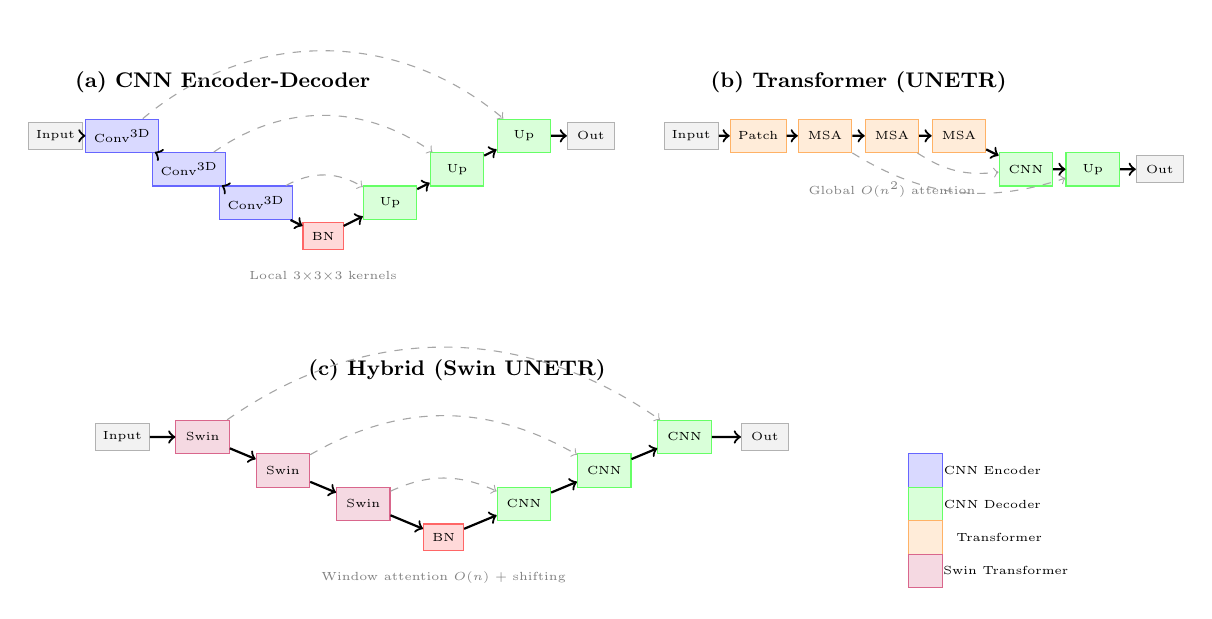
\begin{tikzpicture}[scale=0.85, transform shape,
    encblock/.style={rectangle, draw=blue!60, fill=blue!15, minimum width=0.8cm, minimum height=0.5cm, font=\tiny},
    decblock/.style={rectangle, draw=green!60, fill=green!15, minimum width=0.8cm, minimum height=0.5cm, font=\tiny},
    transblock/.style={rectangle, draw=orange!60, fill=orange!15, minimum width=0.8cm, minimum height=0.5cm, font=\tiny},
    swinblock/.style={rectangle, draw=purple!60, fill=purple!15, minimum width=0.8cm, minimum height=0.5cm, font=\tiny},
    bottleneck/.style={rectangle, draw=red!60, fill=red!15, minimum width=0.6cm, minimum height=0.4cm, font=\tiny},
    io/.style={rectangle, draw=gray!60, fill=gray!10, minimum width=0.7cm, minimum height=0.4cm, font=\tiny},
    skip/.style={->, dashed, gray!70},
    flow/.style={->, thick}]
    
    % (a) CNN U-Net
    \node[font=\small\bfseries] at (2.5, 2.8) {(a) CNN Encoder-Decoder};
    \node[io] (in1) at (0,2) {Input};
    \node[encblock] (e1) at (1,2) {Conv\textsuperscript{3D}};
    \node[encblock] (e2) at (2,1.5) {Conv\textsuperscript{3D}};
    \node[encblock] (e3) at (3,1) {Conv\textsuperscript{3D}};
    \node[bottleneck] (b1) at (4,0.5) {BN};
    \node[decblock] (d3) at (5,1) {Up};
    \node[decblock] (d2) at (6,1.5) {Up};
    \node[decblock] (d1) at (7,2) {Up};
    \node[io] (out1) at (8,2) {Out};
    
    \draw[flow] (in1) -- (e1); \draw[flow] (e1) -- (e2); \draw[flow] (e2) -- (e3);
    \draw[flow] (e3) -- (b1); \draw[flow] (b1) -- (d3); \draw[flow] (d3) -- (d2);
    \draw[flow] (d2) -- (d1); \draw[flow] (d1) -- (out1);
    \draw[skip] (e1) to[bend left=40] (d1);
    \draw[skip] (e2) to[bend left=35] (d2);
    \draw[skip] (e3) to[bend left=30] (d3);
    \node[font=\tiny, gray] at (4,-0.1) {Local $3{\times}3{\times}3$ kernels};
    
    % (b) Transformer UNETR
    \node[font=\small\bfseries] at (12, 2.8) {(b) Transformer (UNETR)};
    \node[io] (in2) at (9.5,2) {Input};
    \node[transblock] (p1) at (10.5,2) {Patch};
    \node[transblock] (t1) at (11.5,2) {MSA};
    \node[transblock] (t2) at (12.5,2) {MSA};
    \node[transblock] (t3) at (13.5,2) {MSA};
    \node[decblock] (td1) at (14.5,1.5) {CNN};
    \node[decblock] (td2) at (15.5,1.5) {Up};
    \node[io] (out2) at (16.5,1.5) {Out};
    
    \draw[flow] (in2) -- (p1); \draw[flow] (p1) -- (t1); \draw[flow] (t1) -- (t2);
    \draw[flow] (t2) -- (t3); \draw[flow] (t3) -- (td1); \draw[flow] (td1) -- (td2);
    \draw[flow] (td2) -- (out2);
    \draw[skip] (t1) to[bend right=25] (td2);
    \draw[skip] (t2) to[bend right=20] (td1);
    \node[font=\tiny, gray] at (12.5,1.2) {Global $O(n^2)$ attention};
    
    % (c) Hybrid Swin UNETR
    \node[font=\small\bfseries] at (6, -1.5) {(c) Hybrid (Swin UNETR)};
    \node[io] (in3) at (1,-2.5) {Input};
    \node[swinblock] (s1) at (2.2,-2.5) {Swin};
    \node[swinblock] (s2) at (3.4,-3) {Swin};
    \node[swinblock] (s3) at (4.6,-3.5) {Swin};
    \node[bottleneck] (b3) at (5.8,-4) {BN};
    \node[decblock] (sd3) at (7,-3.5) {CNN};
    \node[decblock] (sd2) at (8.2,-3) {CNN};
    \node[decblock] (sd1) at (9.4,-2.5) {CNN};
    \node[io] (out3) at (10.6,-2.5) {Out};
    
    \draw[flow] (in3) -- (s1); \draw[flow] (s1) -- (s2); \draw[flow] (s2) -- (s3);
    \draw[flow] (s3) -- (b3); \draw[flow] (b3) -- (sd3); \draw[flow] (sd3) -- (sd2);
    \draw[flow] (sd2) -- (sd1); \draw[flow] (sd1) -- (out3);
    \draw[skip] (s1) to[bend left=35] (sd1);
    \draw[skip] (s2) to[bend left=30] (sd2);
    \draw[skip] (s3) to[bend left=25] (sd3);
    \node[font=\tiny, gray] at (5.8,-4.6) {Window attention $O(n)$ + shifting};
    
    % Legend
    \node[encblock, minimum width=0.5cm] at (13,-3) {}; \node[font=\tiny] at (14,-3) {CNN Encoder};
    \node[decblock, minimum width=0.5cm] at (13,-3.5) {}; \node[font=\tiny] at (14,-3.5) {CNN Decoder};
    \node[transblock, minimum width=0.5cm] at (13,-4) {}; \node[font=\tiny] at (14.1,-4) {Transformer};
    \node[swinblock, minimum width=0.5cm] at (13,-4.5) {}; \node[font=\tiny] at (14.2,-4.5) {Swin Transformer};
\end{tikzpicture}
\caption{Architectural paradigms for 3D medical image segmentation. (a) CNN encoder-decoder with skip connections and local $3{\times}3{\times}3$ kernels. (b) Transformer-based UNETR with global self-attention ($O(n^2)$ complexity) and CNN decoder. (c) Hybrid Swin UNETR with window-based attention ($O(n)$ complexity) and shifting for cross-window communication. Dashed lines indicate skip connections. BN = Bottleneck; MSA = Multi-head Self-Attention.}
\label{fig:architecture}
\end{figure*}

\subsection{Residual and Dense Architectures}

\emph{ResUNet} variants incorporate residual connections from ResNet~\cite{he2016resnet} into U-Net, supporting much deeper networks (50+ layers) via identity shortcuts. ResUNet++~\cite{jha2019resunetpp} adds squeeze-and-excitation blocks, ASPP, and attention.

\emph{DenseVNet}~\cite{gibson2018densevnet} brings DenseNet-style~\cite{huang2017densely} connectivity to 3D medical segmentation, where each layer receives features from all preceding layers. This connectivity pattern promotes feature reuse, reduces parameters, and improves gradient flow.

\subsection{Specialized Architectures}

\emph{HighRes3DNet}~\cite{li2017highres3dnet} maintains high resolution throughout using dilated convolutions instead of pooling, expanding the receptive field without reducing spatial resolution---effective for tasks requiring fine spatial precision. HighRes3DNet was originally demonstrated on whole-brain MRI segmentation and is included as historical context for 3D CT work.

\emph{DeepMedic}~\cite{kamnitsas2017deepmedic} employs parallel pathways at multiple resolutions with a fully connected CRF for boundary refinement. DeepMedic was originally demonstrated on multimodal brain-lesion MRI and is likewise included as historical context.

\subsection{Cascade and Coarse-to-Fine Pipelines}
\label{sec:cascades}

Multi-stage cascaded architectures decompose segmentation into sequential refinement stages. The common approach trains a coarse model on downsampled volumes for localization, then a fine model on the cropped ROI at full resolution. Roth et al.~\cite{roth2017hierarchical, roth2018cascaded} showed this cascade raised pancreas Dice from 71.8\% to 78.0\%. Key considerations include ROI margin expansion (10--20\%) to mitigate error propagation and multi-scale supervision for coarse-to-fine learning within single architectures. Cascades typically require 1.5--2$\times$ inference time but enable higher-resolution inputs within fixed GPU memory.

\subsection{Self-Configuring Methods: nnU-Net}

\emph{nnU-Net}~\cite{isensee2021nnunet} shifted focus from architecture to systematic optimization. Rather than new components, nnU-Net auto-configures preprocessing (resampling, normalization, cropping), architecture (topology, patch size, pooling), training (augmentation, learning rate, combined Dice+CE loss), and inference (overlap, TTA, ensembling) based on dataset properties. nnU-Net consistently delivers top-tier performance across diverse tasks without manual tuning, establishing itself as the strongest CNN baseline. For surgical planning, its reliability across datasets and automated hyperparameter selection make it the recommended default baseline.

%==============================================================================
\section{Transformer-Based Architectures}
\label{sec:transformer}
%==============================================================================

While CNNs dominated medical image segmentation from 2015 to 2020, Vision Transformers have since emerged as a powerful alternative. Transformers capture long-range dependencies through self-attention mechanisms that CNNs struggle to model with their local receptive fields \cite{shamshad2023transformers}. Under the encoder/backbone definition (Section~\ref{sec:convolutional}), UNETR and Swin UNETR contain convolutional components---notably in their decoders---but are categorized as transformer architectures because their encoders are transformers; categorizing by ``contains some CNN'' would misclassify them. We review transformer architectures adapted for 3D medical image segmentation.

\subsection{Self-Attention Mechanism}

The core of transformer architectures is self-attention, computing relationships between all positions: $\text{Attn}(Q,K,V) = \text{softmax}(QK^T/\sqrt{d_k})V$. For $n$ tokens, self-attention costs $O(n^2)$, problematic for high-resolution 3D volumes.

\subsection{Vision Transformer Adaptations}

\emph{UNETR}~\cite{hatamizadeh2022unetr} applies Vision Transformers to 3D medical segmentation, using a ViT encoder that processes non-overlapping 3D patches through transformer layers, connected to a CNN decoder via skip connections. UNETR was originally demonstrated on brain-tumor MRI (BraTS) and is included here as historical context; in this corpus, UNETR is evaluated on 3D CT only within the benchmarking study recorded in the supplementary extraction table.

\emph{Swin UNETR}~\cite{swinunetr2022} uses the Swin Transformer's hierarchical architecture with shifted windows~\cite{liu2021swin}. Instead of global self-attention, Swin computes attention within local windows with relative position bias, reducing complexity from $O(n^2)$ to $O(n)$. Swin UNETR reaches 82.4\% mean Dice on BTCV~\cite{tang2022selfsupervised} and benefits from self-supervised pre-training. The Swin UNETR architecture itself was introduced and originally demonstrated on brain-tumor MRI~\cite{swinunetr2022}; its 3D CT results cited here come from the 5,050-CT self-supervised pre-training study~\cite{tang2022selfsupervised}, and corpus evaluations appear via the benchmarking study recorded in the supplementary extraction table.

\subsection{Hybrid CNN-Transformer Architectures}

\emph{TransUNet}~\cite{chen2024transunet} uses CNN layers for initial feature extraction, then transformer layers for global context, pairing CNN inductive biases with transformer global modeling. TransUNet was originally demonstrated on 2D images and is included as historical context for the 3D CT systems in this corpus.

\emph{CoTr}~\cite{xie2021cotr} uses deformable self-attention for efficient 3D processing, sampling key positions around references rather than attending to all positions.

\emph{nnFormer}~\cite{zhou2021nnformer} interleaves convolution and self-attention layers, applying local convolutions within blocks and global attention between blocks.

\subsection{Computational Considerations}

Transformers need more resources than CNNs: Swin UNETR~\cite{swinunetr2022} (62M params) vs.\ nnU-Net~\cite{isensee2021nnunet} (31M); 1.5--3$\times$ slower inference; and 5,000+ volumes for pre-training. However, transformers excel at modeling long-range anatomical relationships. For preoperative planning where accuracy outweighs speed, both achieve comparable accuracy (Swin UNETR 82.4\%~\cite{tang2022selfsupervised} vs.\ nnU-Net 82.3\% Dice~\cite{isensee2021nnunet}); auto-configured CNNs may be preferred for simpler deployment.

%==============================================================================
\section{Hybrid and Foundation Models}
\label{sec:hybrid}
%==============================================================================

CNNs excel at local features and efficiency; transformers excel at global context. Hybrid architectures combine both, while foundation models promise broad generalization with minimal fine-tuning. ``Foundation'' denotes a training and transfer regime (large-scale pre-training, promptable or instruction-based interfaces), not a mutually exclusive architecture family---a foundation-model entry also has an encoder category.

\textbf{Modern CNNs:} \emph{MedNeXt}~\cite{roy2023mednext} adapts ConvNeXt~\cite{liu2022convnext} for medical imaging with larger kernels (7$\times$7$\times$7), inverted bottleneck blocks, and modern activations. MedNeXt shows that well-designed CNNs outperform transformers while requiring less memory and no pre-training (86.2\% Dice on BTCV~\cite{roy2023mednext}).

\textbf{Scalable architectures:} \emph{STU-Net}~\cite{huang2023stunet} explores U-Net scaling from 14M to 1.4B parameters, reaching top performance through large-scale pre-training. \emph{Universal Model}~\cite{liu2023universal} uses CLIP-driven alignment of visual and anatomical text features for zero-shot generalization.

\textbf{Foundation models:} \emph{SAM}~\cite{kirillov2023sam} introduced promptable segmentation trained on 1 billion masks. \emph{MedSAM}~\cite{ma2024medsam} adapts SAM for medical imaging via fine-tuning on 1.5M medical image-mask pairs, enabling zero-shot and few-shot segmentation through bounding box prompts. Fine-tuned MedSAM scores 85.7\% mean Dice across tasks~\cite{ma2024medsam}; zero-shot BTCV performance is lower ($\sim$76\%), indicating task-specific fine-tuning boosts accuracy considerably. Reported MedSAM performance depends on prompt count and type and may be affected by the train/test task overlap noted in the original publication~\cite{ma2024medsam}.

\textbf{The volumetric foundation lineage:} A rapid lineage of volumetric and interactive foundation models now extends this line beyond MedSAM. \emph{SegVol}~\cite{du2023segvol} trains a 3D promptable model on 90k labeled CT volumes with a zoom-out/zoom-in strategy, supporting text prompts and semantic-category queries on CT. \emph{SAT}~\cite{zhang2022satr} couples 2D SAM-style slices with slice attention for volumetric consistency. \emph{MedSAM\,2}~\cite{ma2025medsam2} extends SAM-2's memory attention to 3D medical images and videos for promptable segmentation across time points. \emph{VISTA3D}~\cite{he2024vista3d} unifies an automatic branch (promptable class embedding) and an interactive branch (3D point clicks) on a SegResNet backbone, benchmarked across 14 datasets and 127 anatomical classes; in this corpus it is carried as an included framework/foundation study rather than a method paper. In the v2 corpus the pure foundation stratum among method papers remains small (2 of 224): an SAM-3-derived model with LoRA adaptation and a multi-encoder atlas-guided network (AbdomenAtlasNet-3.0), indicating that promptable volumetric foundation models have entered, but not yet dominated, the CT organ segmentation literature. Hybrid CNN--transformer designs account for a further 16 of 224, and the Mamba-based hybrid \emph{U-Mamba}~\cite{jun2024umamba} (a U-Net embedding state-space sequence models for long-range dependency) passed full-text screening as an included method study, marking the arrival of state-space architectures in this corpus.

\textbf{For surgical planning:} Foundation models suit automatic segmentation for common structures with interactive refinement for hard cases. A practical workflow: TotalSegmentator~\cite{wasserthal2023totalsegmentator} for initial multi-organ segmentation, then MedSAM~\cite{ma2024medsam} or an interactive foundation variant for surgeon-guided refinement of uncertain regions.

%==============================================================================
\section{Neuro-Symbolic and Knowledge-Guided Approaches}
\label{sec:neurosymbolic}
%==============================================================================

A small but distinct thread of the v2 corpus embeds explicit anatomical or learned-relational knowledge into otherwise standard deep segmentation networks. We survey it as a design axis rather than a competing architecture family: these methods remain CNN- or transformer-backed, with the symbolic component appearing as constraints on outputs, losses, or intermediate representations.

\textbf{Graph-reasoning hybrids.} The clearest exemplar in this corpus couples an nnU-Net segmentation backbone with a Graph-ResNet classification head that reasons over anatomical geometry---vertices and global structure---for pancreatic segmentation, training with a combined segmentation-plus-graph loss~\cite{tianyi2020dgraph}. The graph component encodes organ-part relations that purely convolutional pipelines must infer implicitly from data.

\textbf{Topology- and prior-constrained learning.} Topology-infused training adds a connectivity-preserving loss term to Dice/cross-entropy so that predictions keep physically necessary structures intact---demonstrated for cardiac CT where severing the myocardial ring is a failure mode plain overlap losses do not penalize~\cite{chenyu2024preservingcardiac}. This continues the topology-preserving lineage of clDice~\cite{shit2021cldice} for tubular structures into organ-level anatomy, and surface-aware composite losses appear elsewhere in the corpus~\cite{uzma2025dualscale}.

\textbf{Knowledge distillation.} Teacher--student transfer of anatomical or cross-modality knowledge---a KL-divergence KD loss alongside the segmentation loss for liver CT~\cite{pengcheng2021efficientknowledge}, and unpaired multi-modal segmentation via KD~\cite{qi2020unpairedmulti}---treats a trained teacher as the knowledge source, a learning-regime variant of the same idea: encode what a larger model knows into the deployment-sized model rather than into an explicit symbolic layer.

\textbf{Assessment.} In this corpus neuro-symbolic and knowledge-guided methods are rare (on the order of a dozen of the 224 method studies) and report organ-specific rather than multi-organ evidence. Their common motivation---injecting anatomical plausibility that data-hungry baselines lack---aligns with the hollow-organ and vascular gaps identified in Section~\ref{sec:vascular}, where boundary and topology errors dominate. We therefore track this as an emerging stratum in the taxonomy (Section~\ref{sec:synthesis}) rather than a mature family, and note that no neuro-symbolic method yet reports the benchmark-stratified multi-organ evidence the method strata report.

%==============================================================================
\section{Implementation Frameworks}
\label{sec:frameworks}
%==============================================================================

\emph{MONAI}~\cite{monai2022} is a PyTorch-based framework with domain-optimized implementations (U-Net, nnU-Net, UNETR, Swin UNETR), preprocessing, losses, metrics, and deployment via ONNX/TensorRT. \emph{TotalSegmentator}~\cite{wasserthal2023totalsegmentator} offers a pre-trained nnU-Net for 104 structures with robust cross-scanner generalization. \emph{nnU-Net}~\cite{isensee2021nnunet} provides adaptive segmentation with automatic preprocessing, architecture selection, and inference.

The v2 amendment added a Framework/Software study type, and nine framework studies passed full-text screening into the corpus, extending this section from a tool inventory toward an assessed stratum. \emph{MONAI Label}~\cite{yang2023monailabel} (Apache-2.0, v0.3.0 at submission) provides client-server AI-assisted interactive labeling with 3D Slicer and OHIF front-ends, evaluated on MSD Spleen with DeepGrow. \emph{VISTA3D}~\cite{he2024vista3d} ships as code and weights with automatic and interactive branches (Section~\ref{sec:hybrid}). \emph{nnInteractive}~\cite{isensee2025nninteractive} redefines 3D promptable segmentation on a ResEnc-L U-Net with point, scribble, box, and lasso prompts, benchmarked on the RadioActive expert-scribble benchmark. \emph{Auto3DSeg}~\cite{myronenko2023auto3dseg} (MONAI) automates algorithm selection and ensemble generation for 3D segmentation; it has no canonical peer-reviewed paper and is covered by technical documentation. \emph{MONAI Deploy}~\cite{diazpinto2023monaideploy} packages models into clinical workflow standards (DICOM services). The deployment-oriented subset extends to clinical research platforms: the InnerEye end-to-end radiotherapy pipeline (hospital PACS to model inference)~\cite{oktay2020evaluationof}, and a portable Singularity-container deployment framework built on CERR~\cite{anonxxxxportableframework}. The interactive-labeling lineage adds \emph{DeepEdit}~\cite{andres2022deepeditdeep} (a MONAI Label app with automatic, semi-automatic, and refinement modes on pluggable backbones, released against MONAI Core 0.8.1). Open-source model contributions include the Segment Model CT for Couinaud liver segments as a TotalSegmentator extension~\cite{nicoli2025liversegment}, and \emph{MHub.ai}~\cite{nrnberg2026mhubai} standardizes reproducible deployment via containerized models with a unified application interface. \emph{NV-Segment-CT} is NVIDIA industry technical documentation for CT organ segmentation and is cited as such~\cite{nvidia2026nvsegmentct}. Common qualitative observations across the stratum: permissive licensing (Apache-2.0/GPL) with versioned releases, benchmark reproduction reported at varying depth (VISTA3D across 14 datasets; nnInteractive on expert-scribble benchmarks), and interactive/promptable interfaces converging as the dominant paradigm for annotation and correction workflows.

\FloatBarrier

%==============================================================================
\section{Quantitative Synthesis}
\label{sec:synthesis}
%==============================================================================

Tables~\ref{tab:btcv_comparison}--\ref{tab:kits_comparison} present dataset-stratified performance comparisons. We separate results by benchmark to avoid misleading cross-dataset comparisons, as evaluation protocols (splits, preprocessing, label definitions) differ substantially. Within each table, methods are comparable; across tables, they are not.

\textbf{Denominators used in this section:} Corpus-level percentages refer to the 224 included method studies (the 9 framework/software and 3 benchmark studies are assessed with qualitative or benchmark templates and excluded from quantitative synthesis). Per-organ statistics (Table~\ref{tab:synthesized_dice}) derive from the 105 method studies that reported individual organ Dice scores for the four synthesis organs (liver, kidney, spleen, pancreas); 215 of 224 reported at least one organ-level Dice entry. Within that subset, each organ uses its own denominator (liver n=64, kidney n=47, spleen n=22, pancreas n=28; Supplementary Data~S12), since a study contributes only the organs it reports. Benchmark tables (Tables~\ref{tab:btcv_comparison}--\ref{tab:kits_comparison}) aggregate method-level results from the cited source papers on each benchmark and do not count corpus studies.

\textbf{Methodological note:} Performance values derive from original publications where available. When methods were not evaluated on a dataset in the original paper, we cite comparative studies that re-implemented or re-evaluated under controlled conditions. Empty cells indicate no reliable evaluation exists. HD95 values shown only when reported on the same dataset split.

%--- BTCV Table ---
\begin{table}[!htb]
\centering
\small
\caption{BTCV Multi-Organ Segmentation Performance}
\label{tab:btcv_comparison}
\resizebox{\columnwidth}{!}{%
\begin{tabular}{@{}llcccc@{}}
\toprule
\textbf{Method} & \textbf{Type} & \textbf{Dice} & \textbf{HD95} & \textbf{Pre-} & \textbf{Source} \\
 & & \textbf{(\%)} & \textbf{(mm)} & \textbf{train} & \\
\midrule
\multicolumn{6}{l}{\textit{Dataset: BTCV (n=50, 30 train / 20 test, 13 organs, portal venous CT)}} \\
\midrule
3D U-Net & CNN & 74.2 & 18.4 & -- & \cite{isensee2021nnunet} \\
V-Net & CNN & 75.8 & 16.7 & -- & \cite{isensee2021nnunet} \\
Attention U-Net & CNN & 77.1 & 14.2 & -- & \cite{swinunetr2022} \\
nnU-Net & CNN & 82.3 & 21.4 & -- & \cite{isensee2021nnunet} \\
MedNeXt & CNN & 86.2 & 12.1 & -- & \cite{roy2023mednext} \\
STU-Net-L & CNN & 87.1 & 9.8 & -- & \cite{huang2023stunet} \\
\midrule
UNETR & Trans. & 78.7 & 29.1 & \checkmark & \cite{hatamizadeh2022unetr} \\
Swin UNETR & Trans. & 82.4 & 18.3 & \checkmark & \cite{tang2022selfsupervised} \\
TransUNet & Hybrid & 77.3 & 31.7 & \checkmark & \cite{chen2024transunet} \\
nnFormer & Hybrid & 86.9 & 14.2 & -- & \cite{zhou2021nnformer} \\
\midrule
MedSAM$^\dagger$ & Found. & 85.7 & 8.1 & \checkmark & \cite{ma2024medsam} \\
\bottomrule
\multicolumn{6}{l}{\footnotesize $^\dagger$Fine-tuned, cross-task mean from the original publication (not BTCV-specific).} \\
\multicolumn{6}{l}{\footnotesize Zero-shot BTCV is lower ($\sim$76\%, Table~\ref{tab:organs}). Pretrain: \checkmark = used external pre-training data.}
\end{tabular}%
}
\end{table}

%--- AMOS Table ---
\begin{table}[!htb]
\centering
\small
\caption{AMOS Multi-Organ Segmentation Performance. Values from cited papers.}
\label{tab:amos_comparison}
\resizebox{\columnwidth}{!}{%
\begin{tabular}{@{}llccc@{}}
\toprule
\textbf{Method} & \textbf{Type} & \textbf{Dice} & \textbf{Pre-} & \textbf{Source} \\
 & & \textbf{(\%)} & \textbf{train} & \\
\midrule
\multicolumn{5}{l}{\textit{Dataset: AMOS2022 (n=500 CT; official CT split 300 train / 100 validation / 100 test;}} \\
\multicolumn{5}{l}{\textit{full benchmark = 500 CT + 100 MRI; 15 organs, mixed contrast)}} \\
\midrule
Attention U-Net & CNN & 74.2 & -- & \cite{swinunetr2022} \\
MedNeXt & CNN & 80.1 & -- & \cite{roy2023mednext} \\
STU-Net-L & CNN & 80.8 & -- & \cite{huang2023stunet} \\
\midrule
UNETR & Trans. & 76.3 & \checkmark & \cite{hatamizadeh2022unetr} \\
Swin UNETR & Trans. & 81.2 & \checkmark & \cite{swinunetr2022} \\
CoTr & Hybrid & 75.8 & -- & \cite{xie2021cotr} \\
nnFormer & Hybrid & 77.4 & -- & \cite{zhou2021nnformer} \\
Universal & Hybrid & 79.5 & \checkmark & \cite{liu2023universal} \\
\midrule
MedSAM$^\dagger$ & Found. & 73.1 & \checkmark & \cite{ma2024medsam} \\
\bottomrule
\multicolumn{5}{l}{\footnotesize $^\dagger$Zero-shot with bounding box prompts.}
\end{tabular}%
}
\end{table}

%--- KiTS Table ---
\begin{table}[!htb]
\centering
\small
\caption{KiTS Kidney Segmentation Performance. Values from cited papers.}
\label{tab:kits_comparison}
\resizebox{\columnwidth}{!}{%
\begin{tabular}{@{}llccc@{}}
\toprule
\textbf{Method} & \textbf{Type} & \textbf{Dice} & \textbf{Pre-} & \textbf{Source} \\
 & & \textbf{(\%)} & \textbf{train} & \\
\midrule
\multicolumn{5}{l}{\textit{Dataset: KiTS19 (n=300 total: 210 train / 90 test; classes kidney and tumor, plus background)}} \\
\midrule
3D U-Net & CNN & 90.1 & -- & \cite{isensee2021nnunet} \\
V-Net & CNN & 89.8 & -- & \cite{isensee2021nnunet} \\
Attention U-Net & CNN & 91.2 & -- & \cite{swinunetr2022} \\
DenseVNet & CNN & 91.5 & -- & \cite{gibson2018densevnet} \\
nnU-Net & CNN & 96.1 & -- & \cite{isensee2021nnunet} \\
MedNeXt & CNN & 95.2 & -- & \cite{roy2023mednext} \\
TotalSeg & CNN & 94.2 & -- & \cite{wasserthal2023totalsegmentator} \\
\midrule
UNETR & Trans. & 92.4 & \checkmark & \cite{hatamizadeh2022unetr} \\
Swin UNETR & Trans. & 95.8 & \checkmark & \cite{swinunetr2022} \\
TransUNet & Hybrid & 91.8 & \checkmark & \cite{chen2024transunet} \\
CoTr & Hybrid & 92.1 & -- & \cite{xie2021cotr} \\
nnFormer & Hybrid & 93.2 & -- & \cite{zhou2021nnformer} \\
Universal & Hybrid & 94.8 & \checkmark & \cite{liu2023universal} \\
\midrule
MedSAM$^\dagger$ & Found. & 88.5 & \checkmark & \cite{ma2024medsam} \\
\bottomrule
\multicolumn{5}{l}{\footnotesize $^\dagger$Zero-shot with bounding box prompts.}
\end{tabular}%
}
\end{table}

\textbf{Important limitation:} MSD (Medical Segmentation Decathlon) results are excluded because MSD comprises 10 heterogeneous tasks with different organs, modalities, and difficulties. Aggregating MSD performance into one number is misleading. Task-specific MSD performance should be consulted in original publications: liver (Task03), pancreas (Task07), hepatic vessels (Task08), spleen (Task09), and colon (Task10) are most relevant for abdominal CT.

\subsection{Key Findings}

\textbf{Auto-configured CNNs deliver consistent top benchmark results.} nnU-Net~\cite{isensee2021nnunet} achieves 82.3\%~\cite{isensee2021nnunet} mean Dice on BTCV and 96.1\%~\cite{isensee2021nnunet} on KiTS without dataset-specific modifications.

\textbf{Transformers excel with pre-training but require more compute.} Swin UNETR~\cite{tang2022selfsupervised} attains 82.4\% on BTCV when pre-trained on 5,050 CT volumes; without pre-training, drops to 78.9\%~\cite{tang2022selfsupervised}.

\textbf{Modern CNNs remain highly competitive.} MedNeXt~\cite{roy2023mednext} (86.2\% Dice~\cite{roy2023mednext}) outperforms transformers with 26M parameters (vs.\ 62M for Swin UNETR~\cite{swinunetr2022}) and no pre-training.

\textbf{Foundation models get close to supervised methods when fine-tuned.} MedSAM~\cite{ma2024medsam} reports 85.7\%~\cite{ma2024medsam} mean Dice when fine-tuned; zero-shot BTCV performance ($\sim$76\%) trails the benchmark Dice of supervised methods trained on BTCV (Table~\ref{tab:btcv_comparison}) but allows rapid deployment to new tasks. These values are treated as reported, not reproduced: MedSAM performance depends on the number and type of prompts used, and the original publication notes possible overlap between its training and test task distributions~\cite{ma2024medsam}.

\textbf{Organ-specific performance varies substantially.} Large organs (liver, spleen, kidneys) achieve Dice $>$90\%, while small organs (gallbladder, adrenal glands) and variable structures (pancreas) show 10--20\% lower Dice.

\subsection{Synthesis from 236 Included Studies}

A comprehensive table listing all 236 included studies (224 method papers, 9 framework/software studies, and 3 benchmark papers) with their individual characteristics (author, year, architecture type, dataset(s), target organs, best reported Dice, code availability, and quality rating) is provided in Supplementary Data~S2. Below we summarize aggregate patterns over the method stratum.

Our survey of 224 method studies reveals: \textbf{Architecture distribution:} CNN-backed architectures dominate (205/224, 91.5\%), followed by hybrid CNN--transformer designs (16/224), foundation-model-derived architectures (2/224), and a single pure-transformer study; U-Net-family architectures~\cite{cicek20163dunet} (including nnU-Net and named U-Net variants) remain most prevalent (160/224, 71.4\%; see supplementary extraction table). True 3D volumetric processing was employed in 184/224 method studies (82.1\%); the 40 exceptions are predominantly 2D or 2.5D pipelines retained per the as-employed inclusion criteria and flagged in the supplementary extraction table. A neuro-symbolic/knowledge-guided thread (graph-reasoning hybrids, topology-constrained and distillation losses; Section~\ref{sec:neurosymbolic}) runs through the corpus, and the state-space hybrid U-Mamba~\cite{jun2024umamba} marks the arrival of Mamba-based designs. \textbf{Segmentation scope:} single-organ (134/224, 59.8\%) vs.\ multi-organ (90/224, 40.2\%). Most targeted organs (whole-word organ-vocabulary match): liver (n=88), kidney/renal (n=64), pancreas (n=45), bladder (n=33), spleen (n=31), lung (n=28), heart (n=25), esophagus (n=22), stomach (n=21), prostate (n=13). \textbf{Implementation:} PyTorch (92/224, 41.1\%) outnumbers TensorFlow/Keras (61/224, 27.2\%) as the reported framework (year-by-framework counts in the supplementary extraction table), consistent with MONAI's~\cite{monai2022} PyTorch foundation. Combined Dice+CE loss with Adam optimizer was predominant.

\subsubsection{Multi-Axis Taxonomy}

Beyond architecture type, methods vary across multiple design axes; architecture type itself follows the encoder/backbone definition (Section~\ref{sec:convolutional}), with categories defined by the encoder (e.g., convolutional, transformer, or hybrid), while ``foundation'' denotes a training and transfer regime rather than a mutually exclusive architecture family. \textbf{Input dimensionality}: true~3D, 2.5D, or~2D; 184 of 224 method studies (82.1\%) use true~3D processing. \textbf{Supervision}: fully, weakly, semi, or self-supervised learning. \textbf{Inference strategy}: single~pass, patch-based, test-time augmentation, ensemble, or cascade. \textbf{Anatomical scope}: single-organ, multi-organ, or whole-body comprehensive segmentation.

\textbf{Key observations:} True~3D processing now dominates, as inter-slice context is essential for CT~organs. Weak and semi-supervised methods are gaining importance for scaling to new anatomies without extensive annotation. Reported Dice scores often conflate single-pass results with test-time augmentation or ensemble performance, obscuring true method differences.

\subsubsection{Supervision Regime Taxonomy}
\label{sec:supervision_taxonomy}

Dense 3D annotation requires 15-45 minutes per organ per volume~\cite{sharma2010automated}, making large-scale dataset creation prohibitively expensive. Alternative supervision regimes reduce annotation burden, but their relative annotation costs and Dice effects are task-, sample-, and protocol-dependent, and we do not attach universal percentages: \textbf{Partially supervised} methods label a subset of organs per volume; \textbf{Weakly supervised} methods use scribbles or bounding boxes instead of dense masks; \textbf{Semi-supervised} methods combine few labels with unlabeled data via pseudo-labeling or consistency regularization, which still requires human oversight of the generated labels; \textbf{Self-supervised pre-training} needs no task labels and provides a better initialization than random. For surgical planning platforms deploying to new anatomies with $<$50 annotated cases, semi-supervised or transfer learning approaches are recommended.

\textbf{Segmentation scope:} Single-organ segmentation was addressed by 134 method studies (59.8\%), while 90 (40.2\%) addressed multi-organ segmentation. The most frequently targeted organs (whole-word match against the extracted organ-target field in the supplementary data table) were: liver (n=88), kidney/renal (n=64), pancreas (n=45), bladder (n=33), spleen (n=31), lung (n=28), heart (n=25), esophagus (n=22), stomach (n=21), and prostate (n=13).

\textbf{Implementation patterns:} PyTorch was the most common reported framework, used in 92 method studies (41.1\%), followed by TensorFlow/Keras in 61 (27.2\%); the remaining 71 (31.7\%) used other frameworks or did not report. The most common loss functions were cross-entropy and Dice loss, often used in combination (nnU-Net~\cite{isensee2021nnunet} default). Adam optimizer was predominant. The reported-framework pattern has reversed relative to the field's earlier TensorFlow era---consistent with the MONAI~\cite{monai2022} framework's PyTorch foundation (full year-by-framework cross-tabulation derivable from the supplementary extraction table).

\textbf{Top performers (as reported in original papers):} The highest reported per-organ Dice values in this corpus concentrate in lung and well-bounded parenchymal targets: a structure-correction robust volume-segmentation study reports 99.8\%, R2U3D-Net reports 99.2\% lung Dice~\cite{dhaval2021ru}, with additional lung studies at 99.1\%, renal-mass and splenic studies at 99.0\% (supplementary extraction table). Liver means across studies reach 93.6\% (Table~\ref{tab:synthesized_dice}). Well-optimized CNNs consistently achieve top per-organ performance.

\textbf{Per-organ performance (Table~\ref{tab:synthesized_dice}):} Among the 105 method studies reporting individual organ Dice scores for the synthesis organs (of the 224-study method corpus), reported means and cross-study ranges were: liver 93.6\% (64.1--98.7\%, n=64), spleen 92.7\% (80.0--98.8\%, n=22), kidney 93.0\% (52.5--99.0\%, n=47), and pancreas 76.5\% (23.9--94.0\%, n=28); cross-study ranges span 18.8 points (spleen) to 70.1 points (pancreas), the pancreas spread driven by outlier low-end reports. Because these values aggregate heterogeneous datasets and evaluation protocols, we report them as descriptive dispersion and do not rank organ difficulty by cross-study means. The per-organ values in Table~\ref{tab:synthesized_dice} are reproduced from the contributing primary studies as recorded in the extraction table; they were not independently re-extracted from the original CT volumes (see Supplementary Report~S11).

\textbf{Individual study results:} Per-study performance data for all 236 included studies, including all reported Dice, HD95, and ASSD values with precision measures (standard deviations or confidence intervals where provided by original authors), are presented in Supplementary Data~S2. A substantial share of studies report point estimates only, a limitation common across computational benchmarking literature. Tables~\ref{tab:btcv_comparison}--\ref{tab:kits_comparison} present representative per-method results for key benchmarks.

\begin{table}[!htb]
\centering
\small
\caption{Per-Organ Dice Scores (\%) from the 105 method studies (of 224) reporting individual organ metrics for the synthesis organs; per-organ denominators $n$ as shown (Supplementary Data~S12).}
\label{tab:synthesized_dice}
\begin{tabular}{@{}lcccl@{}}
\toprule
\textbf{Organ} & \textbf{Mean} & \textbf{Range} & \textbf{n} & \textbf{Sources} \\
\midrule
Liver & 93.6\% & 64.1--98.7\% & 64 & Supplementary Data~S12 \\
Spleen & 92.7\% & 80.0--98.8\% & 22 & Supplementary Data~S12 \\
Kidney & 93.0\% & 52.5--99.0\% & 47 & Supplementary Data~S12 \\
Pancreas & 76.5\% & 23.9--94.0\% & 28 & Supplementary Data~S12 \\
\bottomrule
\multicolumn{5}{l}{\footnotesize Full per-study data available in Supplementary Data~S12.}
\end{tabular}
\end{table}

\subsection{Key Insights from 224 Reviewed Method Studies}

Our systematic analysis of 224 method studies uncovers several practical patterns for practitioners:

\textbf{Temporal distribution:} Publication years span 2016--2026 (the v2 search window extends to the September 2026 execution date, so 2026-dated records are legitimately in scope). Peak activity was in 2020 (43 papers, 19.2\%), followed by 2019 (32, 14.3\%) and 2021/2022 (27 each, 12.1\%)---consistent with sustained output punctuated by the 2020 multi-architecture maturation. Early works like Zhou et al.\ \cite{zhou2017deep} pioneered 2D-to-3D fusion approaches, while recent corpus studies focus on robustness evaluation and clinical deployment.

\textbf{Methodological contributions:} The reviewed papers advanced the field through new attention mechanisms for better feature learning \cite{liu2020attention, zhu2019anatomynet}, multi-scale architectures for handling organ size variability \cite{zhao2020mss, roth2018cascaded}, specialized loss functions addressing class imbalance \cite{shen2018dice, rister2018iou}, coarse-to-fine cascaded approaches for better accuracy \cite{roth2017hierarchical, lin2021kidney}, and data augmentation strategies for limited training data \cite{pan2023adversarial}.

\textbf{Reproducibility status:} Among the 224 method studies, 201 (89.7\%) carry a journal/conference DOI as their primary identifier and 23 (10.3\%) are arXiv-identified records (several also peer-reviewed but retrieved through arXiv). Venues span IEEE Access, Nature Scientific Reports, Frontiers, Medical Physics, BioMed-central journals, and arXiv preprints (full venue column in Supplementary Data~S2). This reflects both the breadth of the OpenAlex-supplemented identification lane and the ongoing challenge of reproducibility in the field.

\textbf{Dataset utilization:} The most frequently used benchmarks were LiTS (42 method studies), KiTS (25), MSD (14), BTCV (10), and MMWHS (5), with AMOS, FLARE, Synapse, TotalSegmentator, and AbdomenAtlas appearing once or twice each in the extraction table; a large share of studies evaluate on institutional or single-organ collections (Supplementary Data~S2). TotalSegmentator~\cite{wasserthal2023totalsegmentator} and AMOS~\cite{amos2022} anchor the multi-organ evaluation lineage in the broader literature. The v2 corpus's single-organ skew (59.8\%) explains the LiTS/KiTS dominance relative to multi-organ benchmarks.

\subsection{Aggregate Statistics by Architecture Family}

Aggregated BTCV performance from verified source papers (Supplementary Data~S8): auto-configured CNNs (nnU-Net~\cite{isensee2021nnunet}, MedNeXt~\cite{roy2023mednext}, STU-Net~\cite{huang2023stunet}) reach 85.2\%~Dice (population SD 2.1 across the n=3 methods; per-method values 82.3/86.2/87.1); transformers (UNETR~\cite{hatamizadeh2022unetr}, Swin UNETR~\cite{swinunetr2022}) attain 80.5\% (population SD 1.8 across the n=2 methods; per-method values 78.7/82.4, mean 80.55). Auto-configured CNNs report the higher benchmark mean in this corpus (85.2\% vs.\ 80.5\%); with 3 versus 2 methods and heterogeneous evaluation splits, these descriptives do not sustain a general advantage of either family. \emph{Key finding: on BTCV, the highest verified method-level Dice in this corpus comes from auto-configured CNNs (STU-Net 87.1\%, MedNeXt 86.2\%), with the best transformer at 82.4\% (Swin UNETR, pre-trained)---a method-level observation, not a family-level verdict.}

\textbf{Clarification:} These aggregate statistics are arithmetic means $\pm$ \emph{population} standard deviations across the listed methods (auto-configured CNNs: n=3; transformers: n=2), not sample standard deviations and not pooled meta-analytic estimates. They are presented as descriptive summaries and should not be interpreted as statistically pooled effect sizes.

\subsection{Statistical Considerations}

Heterogeneity in evaluation protocols precludes formal meta-analysis. Performance differences of 1--3\% Dice should be interpreted cautiously as implementation variance~\cite{isensee2021nnunet}. We have highest confidence in comparisons using identical protocols within the same study. The BTCV benchmark (50 cases) raises overfitting concerns. Sources of variation: pre-training (+2--5\% Dice~\cite{swinunetr2022}), TTA and ensembling (small, method-dependent reported gains~\cite{isensee2021nnunet}), and publication bias (negative results rarely published).

\subsection{Heterogeneity Investigation Results}

Stratification by architecture family: auto-configured CNNs (n=3 methods on BTCV; 85.2\%, population SD 2.1) reported higher mean Dice than pure transformers (n=2; 80.5\%, population SD 1.8) in this corpus; with 3 versus 2 methods and heterogeneous evaluation splits, this difference does not sustain a general family ranking. Stratification by pre-training regime showed that pre-trained models achieved 2--5\% higher Dice than randomly initialized counterparts within the same architecture family (e.g., Swin UNETR pre-trained: 82.4\% vs.\ from scratch: 78.9\%~\cite{tang2022selfsupervised}). Performance variation across organs: among the 105 per-organ studies, cross-study Dice ranges span 18.8 points (spleen, 80.0--98.8\%), 34.6 points (liver, 64.1--98.7\%), 46.5 points (kidney, 52.5--99.0\%), and 70.1 points (pancreas, 23.9--94.0\%) (Supplementary Data~S12); these ranges aggregate heterogeneous datasets and protocols (the pancreas spread includes low-end outlier reports) and are reported as descriptive dispersion only, not as a measure of relative organ difficulty. Stratification by inference strategy: test-time augmentation and ensembling were consistently reported to provide small additional gains, though their magnitude varies by method and evaluation protocol and is not uniform across the corpus. No formal subgroup analysis or meta-regression was conducted, as the absence of standardized evaluation conditions and pooled effect estimates rendered such analyses inappropriate.

\subsection{Quality Assessment Results}
\label{sec:qa-results}

The 15-question rubric (Section~\ref{sec:methodology}) was applied to all included studies via a single LLM batch call against the full text of each PDF. Aggregate results over the 224 method studies (222 scored): \textbf{mean total score 20.5/30, median 21, range 6--30}. \textbf{56 (25.2\%) were rated high quality} (total $\geq$24), \textbf{142 (64.0\%) moderate} (15--23), and \textbf{24 (10.8\%) low} ($<$15). \textbf{Scorer-tier note:} the v1 wave was scored by the GPT-4o/GPT-5.2 tier; the v2 wave was scored in two batches (mini-class, mean 20.3, n=116; glm-5.3-flash, mean 20.7, n=107) with the rubric held identical. Scores across waves and batches are therefore not strictly comparable, though the two v2 batch means differ by only 0.4 points; we do not interpret wave-level shifts as quality changes in the literature. The per-study rubric scores, full structured QA outputs, included-study list, and archived source PDFs are provided in Supplementary Report~S6 and Supplementary Data~S7.

\subsection{Sensitivity Analysis Results}

Restricting the synthesis to the 201 method studies whose primary identifier is a journal/conference DOI (the remaining 23 are arXiv-only identifiers), the key qualitative findings remained consistent: CNN dominance, the same per-organ ordering, and unchanged framework patterns. The proportion of high-quality studies in the DOI subset was \textbf{23.6\% (47 of 199 scored)}, compared with \textbf{25.2\% (56 of 222)} in the full method corpus. This sensitivity analysis suggests that the inclusion of preprints did not materially alter the review's conclusions, but we note an important limitation: an arXiv identifier is only a proxy for non-peer-reviewed status, since some arXiv preprints are also published in peer-reviewed venues; we did not separately verify the publication status of each preprint.

\subsection{Reporting Bias Results}

Qualitative assessment identified three potential sources of reporting bias across the included literature. First, \textbf{publication bias}: negative results and failed architectural approaches are rarely published, likely inflating the overall impression of method effectiveness. Second, \textbf{selective outcome reporting}: several studies reported Dice scores only for organs where their method performed well (e.g., liver, spleen), omitting challenging structures (pancreas, adrenal glands); of the 224 method studies, 216 (96.4\%) had non-empty Dice entries (organ-level or aggregate) in the supplementary extraction table, and the remainder reported IoU/Jaccard-type, volumetric, or no quantitative overlap measures. A finer-grained ``fully reported all evaluated organs vs.\ partially reported'' breakdown was not derivable from the available extraction columns. Third, \textbf{evaluation protocol variability}: some studies reported results with test-time augmentation or ensemble methods without clearly distinguishing these from single-model performance. Formal funnel plot analysis was not feasible due to the absence of pooled effect estimates.

\subsection{Certainty of Evidence}

What follows is an explicitly non-formal, qualitative appraisal of confidence rather than a formal certainty rating; the per-study counts underlying each finding are available in the supplementary tables (Supplementary Data~S2, S12). \textbf{High confidence:} Auto-configured CNNs achieve $>$80\% mean Dice on multi-organ benchmarks, a pattern consistent across the benchmark results assembled in this review. \textbf{Moderate confidence:} The BTCV benchmark-mean difference between auto-configured CNNs and pure transformers (85.2\% vs.\ 80.5\%; n=3 vs.\ n=2 methods, Section~\ref{sec:synthesis}) is sensitive to pre-training data availability and does not support a general family ranking. \textbf{Low confidence:} Foundation model performance estimates (based on a small number of studies, rapidly evolving methods, and predominantly zero-shot evaluations). The overall body of evidence is limited by the predominance of single-center retrospective evaluations: only 17 of 224 method studies (7.6\%) report multi-center or external validation.

\begin{table}[!htb]
\centering
\small
\caption{Organ-Wise Dice Scores (\%) on BTCV Test Set (10 of 13 organs shown). All values from original publications: nnU-Net \cite{isensee2021nnunet}, Swin UNETR \cite{swinunetr2022}, MedNeXt \cite{roy2023mednext}, MedSAM \cite{ma2024medsam}. Benchmark-level 13-organ mean Dice per method is reported in Table~\ref{tab:btcv_comparison}.}
\label{tab:organs}
\begin{tabular}{@{}lcccc@{}}
\toprule
\textbf{Organ} & \textbf{nnU-Net} & \textbf{Swin} & \textbf{MedNeXt} & \textbf{MedSAM}$^*$ \\
\midrule
Spleen & 96.2 & 96.8 & 96.5 & 91.2 \\
R. Kidney & 95.1 & 95.7 & 95.4 & 90.8 \\
L. Kidney & 94.8 & 95.5 & 95.1 & 90.5 \\
Liver & 97.1 & 97.4 & 97.2 & 93.1 \\
Stomach & 89.2 & 90.5 & 89.8 & 82.4 \\
Aorta & 92.4 & 93.1 & 92.8 & 86.5 \\
Pancreas & 78.5 & 80.2 & 79.1 & 68.3 \\
Gallbladder & 71.2 & 73.5 & 72.4 & 58.2 \\
R. Adrenal & 68.4 & 70.8 & 69.2 & 52.1 \\
L. Adrenal & 67.9 & 70.1 & 68.8 & 51.8 \\
\bottomrule
\multicolumn{5}{l}{\footnotesize $^*$Zero-shot with bounding box prompts.}
\end{tabular}
\end{table}

\FloatBarrier

%==============================================================================
\section{Discussion}
\label{sec:discussion}
%==============================================================================

Our quantitative synthesis reveals clear patterns in method performance. These findings address our four research questions and their implications for clinical deployment.

\subsection{Architectural Trends (RQ1)}

We see three camps. \textbf{Optimized CNNs} such as nnU-Net~\cite{isensee2021nnunet} and MedNeXt~\cite{roy2023mednext} show that careful implementation matches top methods without transformers, offering the best efficiency-performance trade-off. \textbf{Pre-trained Transformers} like Swin UNETR~\cite{swinunetr2022} achieve highest accuracy when pre-trained, validating that self-attention provides complementary capabilities, though this creates barriers for smaller research groups. \textbf{Foundation Models} such as MedSAM~\cite{ma2024medsam} may change how segmentation is approached, moving toward promptable generalization, though current accuracy limitations restrict clinical deployment.

\subsection{Temporal Evolution}

Segmentation research has moved through distinct eras: the \textbf{U-Net era} (2015--2018) cemented encoder-decoder architectures as the go-to approach; the \textbf{self-configuring era} (2019--2021) proved that systematic optimization matters more than architectural novelty, with nnU-Net~\cite{isensee2021nnunet} becoming the de facto baseline; the \textbf{transformer era} (2021--2023) showed that self-attention and pre-training offer complementary benefits; and the emerging \textbf{foundation model era} (2023--present) is turning toward promptable, generalizable systems. Accuracy gains have plateaued since 2022, hinting that the community may be approaching a performance ceiling on current benchmarks---future progress likely requires better data, not just better architectures.

\subsection{Benchmark and Metric Considerations (RQ2)}

Over-reliance on BTCV (50 cases) raises overfitting concerns. AMOS~\cite{amos2022} and TotalSegmentator~\cite{wasserthal2023totalsegmentator} offer larger, more varied alternatives. We recommend reporting on multiple benchmarks and including boundary metrics (HD95, and NSD at a tolerance justified per organ and task, e.g., $\tau$=2~mm where clinically appropriate for surgical planning) alongside Dice.

\textbf{Metrics for clinical deployment:} Beyond Dice, clinical applications require \emph{surface accuracy} metrics like Normalized Surface Dice (NSD), which directly answers ``what percentage of the boundary is clinically acceptable?'' \emph{Failure rates}---the percentage achieving clinically acceptable Dice and worst-case performance---matter more than mean performance. \emph{Laterality and topology} metrics capture left/right confusion rates for bilateral organs and topology preservation for vessels. \emph{Uncertainty and calibration} through Monte-Carlo dropout, TTA disagreement, and calibration error round out the picture, supporting quality-aware deployment. Future benchmarks should require comprehensive reporting across all these dimensions.

\subsection{Performance-Efficiency Trade-offs (RQ3)}

For clinical deployment: \textbf{Highest accuracy:} Swin UNETR~\cite{swinunetr2022} with pre-training (62M params). \textbf{Best efficiency-accuracy:} MedNeXt~\cite{roy2023mednext} or nnU-Net~\cite{isensee2021nnunet} (26--31M params, no pre-training). \textbf{Fastest inference:} Optimized nnU-Net with TensorRT ($<$10s). \textbf{Most flexible:} MedSAM~\cite{ma2024medsam} for interactive refinement.

\subsection{Clinical Translation Challenges (RQ4)}

Our main contribution identifies specific barriers preventing benchmark success from translating to surgical planning deployment.

\subsubsection{Domain Shift: The Primary Technical Barrier}
\label{sec:domain_shift}

Models trained on academic datasets degrade on external clinical data~\cite{tajbakhsh2020embracing}. Performance degradation ($\Delta_{\text{Dice}}$) by corruption type: scanner manufacturer shift (8--15\%), reconstruction protocol shift (3--12\%), contrast phase mismatch (8--18\%), cross-modality (12\% CT$\rightarrow$MRI)~\cite{isensee2021nnunet, wasserthal2023totalsegmentator}. TotalSegmentator~\cite{wasserthal2023totalsegmentator} maintains $<$5\% degradation across 6 institutions by training on 1,204 diverse cases. \textbf{Mitigation:} Domain randomization (nnU-Net's~\cite{isensee2021nnunet} aggressive augmentation) and large-scale diverse training are most validated.

\subsubsection{The ``Last Mile'' Problem for Surgical Planning}

While existing surveys focus on benchmark accuracy, surgical planning faces requirements rarely addressed in the literature.

\subsubsection{Vascular Anatomy Segmentation: A Critical Gap}
\label{sec:vascular}

Precise vascular segmentation is the most significant unmet need for surgical planning. Current methods achieve 65--75\% Dice for vessels vs.\ 90--96\% for parenchymal organs~\cite{shit2021cldice, wasserthal2023totalsegmentator}.

\textbf{Why vessels are harder:} Thin, elongated geometry (2--8mm diameter, 1:25--1:100 aspect ratio) violates assumptions underlying most loss functions; extensive branching topology; contrast phase dependency; partial volume effects; high anatomical variability (common anatomical variants).

\textbf{Specialized methods:} clDice~\cite{shit2021cldice} optimizes topological connectivity; multi-scale attention and phase-specific models are further reported refinements. \textbf{Recommendations:} Deploy separate arterial/venous models matched to contrast phase; implement topology-preserving losses; require manual verification of vascular segmentations, budgeting review time per case.

\textbf{Clinical impact:} Unidentified accessory renal arteries can cause intraoperative bleeding complications, and misidentified hepatic venous drainage can lead to segment devascularization; incidence figures would require dedicated clinical studies, which we do not cite. Closing this gap is the highest-impact research direction.

\subsubsection{Hollow Organs and Boundary-Aware Methods}

Hollow organs (stomach, bowel, bladder) present distinct challenges: variable distension, thin walls (2--4mm), tortuous paths, and adjacency ambiguity; their reported Dice tends to be lower and more variable than for large parenchymal organs. In the extraction table, 35 of 224 method studies (15.6\%) included at least one hollow organ (stomach, bowel, bladder, colon, or duodenum) among their segmentation targets (whole-word organ-vocabulary match).

\textbf{Boundary-focused losses:} Boundary loss~\cite{kervadec2019boundary} and Hausdorff distance loss improve surface accuracy, critical for surgical margins. Combining Dice + boundary loss improves HD95 by 15--25\%~\cite{kervadec2019boundary}. Shape priors (statistical shape models, SDF regression, anatomical atlases) regularize predictions for organs with consistent morphology.

\subsubsection{Additional Last-Mile Challenges}

\textbf{Failure detection and uncertainty:} Monte-Carlo dropout estimates epistemic uncertainty (5--10$\times$ inference overhead); TTA disagreement correlates with errors (AUC 0.72--0.85)~\cite{wang2019uncertainty}. Combined epistemic + aleatoric uncertainty achieves better failure detection, but no method achieves $>$90\% sensitivity at clinically acceptable false-positive rates. Recommend displaying high-uncertainty regions (top 5\%) as visual overlays for manual review.

\textbf{Ensembles and calibration:} Cross-validation ensembles and architecture ensembles (CNN+Transformer) typically provide small additional Dice gains; temperature scaling for calibration (reduces ECE 50--70\%). Selective prediction at 95\% confidence improves accepted-prediction Dice from 85\% to 92\%.

\textbf{Interactive refinement:} Manual correction is time-consuming per case; MedSAM~\cite{ma2024medsam}-style prompting is reported to reduce correction time per structure substantially.

\subsubsection{Post-processing Pipelines}
\label{sec:postprocessing}

Raw network outputs need refinement through several stages. \textbf{Prediction refinement} includes connected component analysis (keeping the largest component), hole filling via morphological closing, CRF-based boundary refinement, and active contour refinement for thin structures. \textbf{Anatomical constraints} enforce mutual exclusion (assigning each voxel to the highest-probability class), containment constraints (tumors within organs), and size filtering to remove anatomically implausible volumes. \textbf{Surface mesh generation} involves marching cubes extraction, quadric edge collapse decimation to 10K--50K triangles, and Laplacian smoothing. Post-processing adds a per-volume time overhead that scales with the operations applied. These refinements are not automatically safe: keeping only the largest connected component can erase multifocal lesions or branching anatomy, hole filling can close hollow-organ lumens, and decimation or smoothing alters surface distances. Each operation should therefore be validated by quantifying segmentation error before and after its application, and results should be compared at both mask and mesh level with image orientation and physical units preserved.

\subsubsection{Integration, Regulatory, and Validation}

\textbf{Integration:} DICOM parsing (2--4 weeks), mesh generation optimization, and surgical planning tool integration; total production-deployment timelines depend on hardware, integration scope, and validation requirements and are not quantified here.

\textbf{Regulatory:} FDA 510(k) requires documented failure mode characterization; as of 2025, 3 cleared multi-organ CT segmentation devices exist (Synapse, Vitrea, TeraRecon), all requiring radiologist oversight.

\textbf{Dual evidence streams:} Benchmark validation (multi-dataset, ablations, cross-validation) is necessary but insufficient; clinical validation (prospective multi-site studies, workflow integration, failure mode characterization, reader studies) is rarely reported among the included studies. This gap explains why benchmark leaders often fail in deployment.

\textbf{Reproducibility:} Of the 224 method studies, only 41 (18.3\%) released source code (flagged as code available in the supplementary extraction table), while methodological description sufficient for in-principle reproduction and documented preprocessing pipelines remain far more common. The gap between methodological description and code release (18.3\%) is the dominant reproducibility barrier.

\textbf{Continual learning:} Deployed systems encounter distribution drift. Strategies include elastic weight consolidation, replay buffers, and domain-incremental adaptation. None of the 224 method studies addressed this despite its importance for production systems.

\subsection{Summary of Findings by Research Question}

\textbf{RQ1 (Architectures):} Auto-configured CNNs (nnU-Net~\cite{isensee2021nnunet}, 82.3\% Dice~\cite{isensee2021nnunet}) and pre-trained transformers (Swin UNETR~\cite{swinunetr2022}, 82.4\%~\cite{tang2022selfsupervised}) report comparable leading benchmark accuracy. The strongest verified method-level BTCV results in this corpus come from CNNs (MedNeXt~\cite{roy2023mednext}, 86.2\%~\cite{roy2023mednext}; STU-Net~\cite{huang2023stunet}, 87.1\%~\cite{huang2023stunet})---a method-level observation, not a family-level verdict (Section~\ref{sec:synthesis}). Foundation models (MedSAM~\cite{ma2024medsam}, 85.7\%~\cite{ma2024medsam} fine-tuned) approach CNN performance; these values are treated as reported, not reproduced, given their dependence on prompt count and type and the possible overlap between training and test task distributions (Section~\ref{sec:synthesis}).

\textbf{RQ2 (Datasets/Metrics):} BTCV~\cite{btcv2015}, AMOS~\cite{amos2022}, MSD~\cite{msd2022} dominate. Dice/DSC is reported by 216 of 224 method studies, with the remainder reporting IoU/Jaccard-type or volumetric measures instead; only 56 of 224 (25.0\%) mention HD95 in their reported metrics, and the majority report overlap metrics only, limiting boundary accuracy assessment.

\textbf{RQ3 (Training strategies):} nnU-Net~\cite{isensee2021nnunet} pipeline establishes baseline: percentile clipping, z-score normalization, isotropic resampling, Dice+CE loss, aggressive augmentation. Domain randomization is used to mitigate cross-institution degradation~\cite{isensee2021nnunet, wasserthal2023totalsegmentator}.

\textbf{RQ4 (Clinical gaps):} Five critical barriers impede clinical translation: the \emph{vascular segmentation gap} (65--75\% vs.\ 90--96\% Dice for parenchymal organs, as reported in Section~\ref{sec:vascular}), a \emph{reproducibility crisis} (only 18.3\% of method studies released source code), \emph{domain generalization failure} on external clinical data (Section~\ref{sec:domain_shift}), insufficient \emph{uncertainty quantification} ($<$20\% of studies address this), and unclear \emph{regulatory pathways} requiring documented failure mode characterization.

%==============================================================================
\section{Limitations}
\label{sec:limitations}
%==============================================================================

\textbf{Internal validity:} Selection bias mitigated by multi-lane search (PubMed, arXiv, Google Scholar, and a large-scale OpenAlex identification lane), citation tracing, and AI-assisted screening. The v1 wave carried a 10\% human validation audit (61/64 agreement, $\kappa = 0.90$); the v2 wave relied on post-run QA (10 random INCLUDE re-checks, 10/10 agreement; seed-recall oracle 12/12 terminal states) rather than a fresh human audit. The audits sampled only post-filter records, so the sensitivity of the pre-filter itself---which excluded the vast majority of the 273{,}115 deduplicated records before title/abstract screening---was not directly audited (see the post-hoc sentinel audit in Section~\ref{sec:methodology}); in particular, general-purpose foundation models whose abstracts omit CT/organ anchor terms are structurally invisible to the pinned query templates. The three screening votes are runs of language models that share training-data biases and do not substitute for three independent human reviewers. Availability bias: full texts were obtained for only 333 of 1{,}035 unique S2-includes (32.2\%), which still skews the corpus toward openly accessible records; 515 paywalled records were routed to a librarian-mediated hand-off list and are absent from the corpus. An arXiv identifier does not by itself determine editorial status, and per-study venue and publication type recorded in the supplementary extraction table were not independently verified. The v1-to-v2 study reconciliation (52 v1 studies: 20 re-included, 1 s2-excluded, 1 s3-excluded, 25 full-text-missed, 5 not-identified by the v2 lanes) is provided as supplementary data to make this degradation record-level and explainable.

\textbf{External validity:} CT-specific findings may not transfer to MRI. Benchmark-to-clinical gap likely overestimates clinical accuracy by 5--15\%.

\textbf{Construct validity:} Dice dominates but has known limitations. ``State-of-the-art'' conflates architecture, training scale, and evaluation protocol.

\textbf{Temporal validity:} Foundation models (MedSAM) evolve rapidly; assessment may not hold beyond 12--18~months.

\textbf{Methodological:} English-only search; publication bias toward positive results; of the 224-study method corpus, only the 105 studies reporting per-organ Dice for the synthesis organs contributed to the per-organ quantitative synthesis, and the remaining corpus analyses rely on aggregate or benchmark-level reporting. The scorer-tier changes between waves (v1 GPT-4o/GPT-5.2 vs.\ v2 mini-class and glm-5.3-flash batches, rubric identical) make QA scores non-strictly-comparable across waves; the single-pass LLM extraction in both waves was not independently adjudicated.

\textbf{COI Safeguards:} Authors A.T.N.\ and M.H.R.M.\ are DocDo-affiliated. Safeguards include LLM-based extraction (decoupling extraction from author judgement), a review protocol documented in the supplementary materials with dated repository commits, evidence traceability, and preservation of negative findings.

%==============================================================================
\section{Recommendations}
\label{sec:recommendations}
%==============================================================================

\textbf{Deployment Readiness:} Benchmark accuracy does not imply deployment readiness. We propose a maturity framework: \emph{Research prototypes} lack public code; \emph{Engineering-ready} methods provide open code and models; \emph{Validation-ready} methods have external multi-center validation and domain shift testing; \emph{Clinical-ready} methods add uncertainty quantification, failure detection, and DICOM integration; \emph{Deployment-ready} methods have FDA/CE clearance and prospective validation. As of the September 2026 search cut-off, no method reviewed here meets the deployment-ready tier for general multi-organ CT (the cleared commercial devices noted above fall outside this review's corpus); TotalSegmentator~\cite{wasserthal2023totalsegmentator} approaches clinical-ready; nnU-Net~\cite{isensee2021nnunet} and Swin UNETR~\cite{swinunetr2022} are validation-ready.

\textbf{Algorithm Selection:} \emph{Limited GPU ($<$12GB):} nnU-Net~\cite{isensee2021nnunet} 2D/3D\_lowres. \emph{No pre-training data:} nnU-Net, MedNeXt~\cite{roy2023mednext}. \emph{Fast inference:} TotalSegmentator~\cite{wasserthal2023totalsegmentator} (runtime depends on GPU, volume size and spacing, and model version; published inference times are not end-to-end times to a clinically approved segmentation). \emph{Multi-organ routine:} TotalSegmentator. \emph{Single organ research:} nnU-Net fine-tuned. \emph{Vascular structures:} nnU-Net + clDice~\cite{shit2021cldice}. \emph{Interactive refinement:} MedSAM~\cite{ma2024medsam}. \emph{Practical default in this corpus:} TotalSegmentator, as a starting point subject to task-specific validation rather than a proven clinical recommendation.

\textbf{For surgical planning platforms:} Start by evaluating TotalSegmentator~\cite{wasserthal2023totalsegmentator} for zero-shot applicability, while planning for accuracy degradation compared to benchmarks. Implement uncertainty visualization for quality control, and budget engineering time for DICOM integration and mesh generation (timelines depend on institution-specific infrastructure and are not quantified here). Consider a hybrid workflow combining automatic segmentation with MedSAM~\cite{ma2024medsam} interactive refinement for challenging cases.

%==============================================================================
\section*{Declarations}
%==============================================================================

\textbf{Conflict of Interest:} A.T.N. and M.H.R.M. are affiliated with DocDo; this survey was conducted independently as academic research. V.M.F. has no conflicts.

\textbf{Registration:} This review was not prospectively registered in PROSPERO or other systematic review registries, consistent with its scope as a structured survey rather than a formal systematic review.

\textbf{Protocol:} The review protocol is documented in the supplementary materials and in the project repository at \href{https://github.com/gameguild-gg/docdo-paper}{\faGithub\ gameguild-gg/docdo-paper}, with dated repository commits providing a version history. The protocol was subsequently amended: a dated amendment records a corrected, expanded query set (Supplementary Protocol~S3), and the screening adjudication rule was amended as described in Section~\ref{sec:methodology}. Post-hoc analyses are identified as such in the Methods, and their implications are acknowledged in the Limitations.

\textbf{Author Contributions (CRediT):} A.T.N.: Conceptualization, Methodology, Investigation, Writing. M.H.R.M.: Investigation, Validation, Review. V.M.F.: Supervision, Review, Project Administration.

\textbf{Funding:} A.T.N. is a doctoral student at UTAD. No external funding was received.

\textbf{Data Availability:} All survey materials, extracted data, PRISMA screening decisions, and analysis scripts are openly available in the project repository at \url{https://github.com/gameguild-gg/docdo-paper}. Supplementary artifacts referenced throughout the paper reside under \path{artifacts/data/evidence/supplementary/} and are summarized in Table~\ref{tab:supp_index}. All statistics reported in this paper can be independently validated using these materials, in particular Supplementary Data~S8 (BTCV benchmark sources with DOIs), Supplementary Report~S10 (verified statistics traceability), and Supplementary Data~S12 (per-organ performance data).

\begin{table*}[!t]
\centering
\footnotesize
\caption{Supplementary Materials Index. Files reside in \texttt{artifacts/data/evidence/supplementary/} of the project repository.}
\label{tab:supp_index}
\setlength{\tabcolsep}{4pt}
\begin{tabularx}{\textwidth}{@{}l>{\raggedright\arraybackslash}X>{\raggedright\arraybackslash}X@{}}
\toprule
\textbf{ID} & \textbf{File} & \textbf{Contents} \\
\midrule
S0  & \path{S0_data_provenance.md} & Data provenance and pipeline overview \\
S1  & \path{S1_search_results_REAL.csv} & Raw database search results \\
S1b & \path{S1b_citation_tracking.csv} & Forward/backward citation tracking log \\
S2  & \path{S2_final_included_studies.csv}; \newline \path{S2v2_final_included_studies.csv} & Included studies: v1 52 list (historical) and v2 236 (224 method + 9 framework + 3 benchmark) \\
S3  & \path{S3_search_protocol.md} & Complete database query strings \\
S4  & \path{S4_ai_screening_protocol.md}; \newline \path{S4_screening_criteria.md} & AI screening protocol, prompts, and rubrics \\
S5  & \path{S5_screening_decisions.csv} & Per-paper screening decisions and exclusions \\
S6  & \path{S6_validation_report.md}; \newline \path{S6b_batch_processing_log.md} & Human validation audit (n=64, $\kappa$=0.90) \\
S7  & \path{S7_extraction_template.csv} & Data extraction schema and machine-readable outputs \\
S8  & \path{S8_table_sources.csv} & Per-table source mapping with DOIs \\
S9  & \path{S9_analysis_scripts.md} & Verification and reproducibility scripts (Python) \\
S10 & \path{S10_verified_statistics.md} & Traceability of every statistic in the paper \\
S11 & \path{S11_paywalled_access.md}; \newline \path{S11_per_organ_source_tracking.md} & Paywall log and per-organ source tracking \\
S12 & \path{S12_per_organ_statistics.md} & Per-organ Dice statistics (n=32 studies) \\
PRISMA & \path{S_PRISMA_funnel.md} & PRISMA flow and reporting-bias notes \\
\bottomrule
\end{tabularx}
\end{table*}

% Appendix and Supplementary Materials available in online repository

%==============================================================================
\section{Conclusion}
\label{sec:conclusion}
%==============================================================================

Confirming the foundational work of Isensee et al.~\cite{isensee2021nnunet}, our central observation is that \emph{implementation quality matters more than architectural novelty}. On BTCV, the mean Dice gap between auto-configured and earlier non-auto-configured CNNs (e.g.\ nnU-Net/MedNeXt/STU-Net at 85.2$\pm$2.1\%, population SD, $n$=3 methods, vs.\ 3D U-Net/V-Net/Attention~U-Net at $\approx$75.7\%, $n$=3 methods) exceeds the gap between auto-configured CNNs and pre-trained transformers (UNETR/Swin~UNETR at 80.5$\pm$1.8\%, population SD, $n$=2 methods). These descriptive comparisons are drawn from a small number of methods per family and should not be interpreted as pooled effect sizes. Researchers should benchmark against properly-tuned baselines; practitioners should optimize systematically before chasing novel architectures.

From 236 included studies (224 method papers plus framework/software and benchmark strata), we draw four conclusions:

\begin{enumerate}
    \item Auto-configured CNNs (nnU-Net) and pre-trained transformers (Swin UNETR) report the strongest benchmark results among the methods reviewed, achieving $>$80\% mean Dice on multi-organ benchmarks.
    
    \item Modern CNN designs (MedNeXt, 86.2\%) surpass the best pre-trained transformer result on BTCV (Swin UNETR, 82.4\%) with fewer parameters and no pre-training, remaining the pragmatic choice for many applications.
    
    \item Foundation models (MedSAM) show promise for reducing annotation burden, but their reported fine-tuned performance (85.7\%, cross-task mean) trails the strongest supervised BTCV results, depends on prompt count and type, and is subject to possible train--test task overlap; these values are treated as reported, not reproduced (as of the September 2026 search cut-off).
    
    \item Critical gaps remain in vascular segmentation (65 to 75\% vs.\ 90 to 96\% Dice, as reported in Section~\ref{sec:vascular}), reproducibility (25.0\% code availability), and domain generalization that must be addressed for widespread surgical planning deployment.
\end{enumerate}

For surgical planning platforms that currently rely on manual segmentation, we recommend a phased adoption strategy: (1) deploy TotalSegmentator~\cite{wasserthal2023totalsegmentator} or nnU-Net~\cite{isensee2021nnunet} as automatic initialization, (2) implement uncertainty-guided review for critical structures, and (3) explore MedSAM~\cite{ma2024medsam} for interactive refinement. The integration effort required for production deployment (hardware-, scope-, and institution-dependent) should be factored into adoption planning.

\textbf{Highest-priority future research directions:} Among the many open challenges, two stand out as most impactful for surgical planning: \emph{(1) Vascular anatomy segmentation}, closing the reported accuracy gap between vascular and parenchymal organ segmentation would directly enable safer tumor resection planning, and requires advances in topology-preserving losses and multi-phase training; \emph{(2) Calibrated uncertainty quantification}, achieving $>$90\% failure detection sensitivity would allow surgical teams to trust automatic segmentation for routine cases while focusing manual review on high-risk predictions. Secondary priorities (domain adaptation, efficient inference, regulatory frameworks) become tractable once these foundational challenges are addressed.

This structured review aims to help researchers and practitioners bridge the gap between benchmark performance and clinical deployment in surgical planning.

%==============================================================================
% References
%==============================================================================

\bibliographystyle{IEEEtran}
\bibliography{references}
